\documentclass[10pt,letterpaper]{article}

\usepackage{amsmath}
\usepackage{}
% \usepackage{mathbb}
% \usepackage[amsmath]{ntheorem}
\usepackage{amsfonts}
\usepackage{graphicx}
\usepackage{fullpage}
\usepackage{hyperref}
% \usepackage[export]{adjustbox}
\usepackage[caption=false]{subfig}

\DeclareMathOperator*{\argmax}{arg\,max}
\DeclareMathOperator*{\argmin}{arg\,min}
\newtheorem{definition}{Definition}
\newtheorem{example}{Example}

\newcommand{\funman}{FUNMAN}
\newcommand{\region}{\bf X}
\newcommand{\posregion}{{\region}^+}
\newcommand{\negregion}{{\region}^-}
\newcommand{\irrelevantregion}{{\region}^\oslash}
\newcommand{\point}{{\bf x}}
\newcommand{\model}{{\bf M}}
\newcommand{\query}{{\bf Q}}
\newcommand{\bounds}{{\bf B}}
\newcommand{\parameters}{{\bf p}}
\newcommand{\parameterbox}{{\bf p}^{[]}}
\newcommand{\reals}{{\mathbb{R}}}

% \setlength{\floatsep}{ 1.0pt plus 2.0pt minus 2.0pt}

\title{\funman Abstraction}
\author{Dan Bryce}
\begin{document}
\maketitle

\section{Introduction}

We describe methods to stratify and abstract (de-stratify) Petrinets for compartmental models.  The motivation for abstracting a Petrinet is to reduce its size, which becomes exponential in the number of stratified variables.  Reducing the size of the model can have a significant impact on runtime, and it is possible to answer useful queries with the abstract model.  The following sections include a background (defining the models), a description of abstraction, an approach needed to bound the abstracted models (or to perform parameter synthesis directly in a simulator), and then a comparison of simulation results for several variations of a baseline model that applies stratification, bounding, and abstraction.  

\section{Background}
\begin{definition}
	A Petrinet $\Omega$ is a directed graph $(V, E)$ with vertices $V=(V_x,
		V_z)$ partitioned into sets $V_x$ of state vertices and $V_z$ of transition
	vertices, and edges $E=(E_{out}, E_{in})$ partitioned into collections $E_{out}$ of
	flow-out and $E_{in}$ flow-in edges (relative to state vertices).
\end{definition}



\begin{definition}
	A flow-out edge $e \in E_{out}$ comprises a pair of vertices $(v_x,v_z)$, where
	$v_x \in V_x$ is a state vertex, $v_z \in V_z$ is a transition vertex, and the
	flow is directed from $v_x$ to $v_z$.
\end{definition}

\begin{definition}
	A flow-in edge $e \in E_{in}$ comprises a pair of vertices $(v_z,v_x)$,
	similar to a flow-out edge, except that the flow is directed from $v_z$ to
	$v_x$.
\end{definition}

\begin{example}
	The SIR model that stratifies the $S$ state variable into $S_1$ and $S_2$
	for two susceptible populations and defines $\Omega$ by:
	\begin{eqnarray*}
		V_x &=& \{v_{S_1}, v_{S_2}, v_{I}, v_{R}\}\\
		V_z &=& \{v_{inf_1}, v_{inf_2}, v_{rec}\}\\
		E_{in} &=& ((v_{inf_1}, v_{S_1}), (v_{inf_1}, v_{I}), (v_{inf_1}, v_{I}), (v_{inf_2}, v_{S_2}), (v_{inf_2}, v_{I}),
		(v_{inf_2}, v_{I}), (v_{rec}, v_{R}))\\
		E_{out} &=& ((v_{S_1}, v_{inf_1}), (v_{S_2}, v_{inf_2}),(v_{I}, v_{inf_1}), (v_{I}, v_{rec}))
	\end{eqnarray*}
\end{example}

\begin{figure}
	\centering    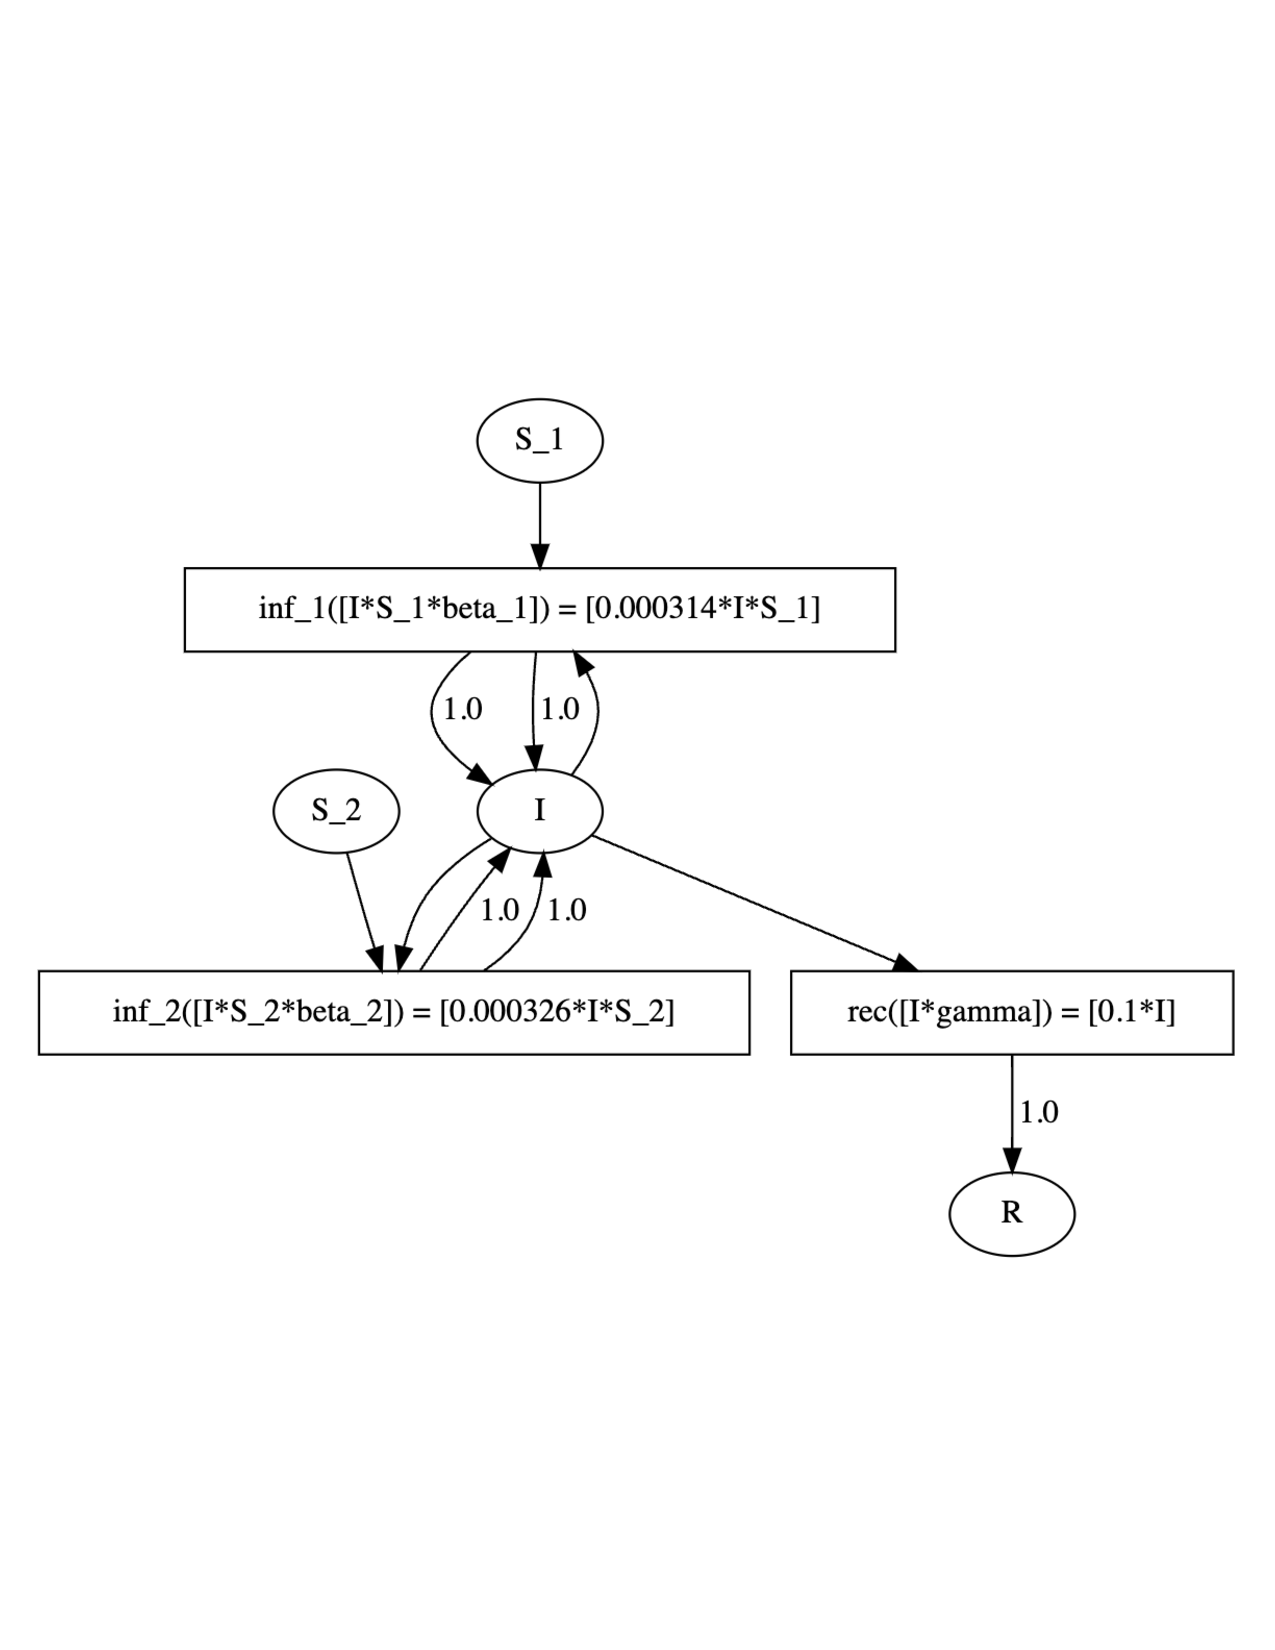
\includegraphics[width=.5\linewidth]{fig/sir/sir_stratified_model.pdf}
	\caption{\label{fig:sir_stratified_model} SIR model stratified with two
		populations in the $S$ state ($S_1$ and $S_2$), each with a unique $\beta$
		parameter ($\beta_1$ and $\beta_2$).}
\end{figure}

\begin{definition}
	The ODE semantics $\Theta$ of the Petrinet $\Omega$ defines a tuple $(P, X,
		Z, {\cal I}, {\cal P}, {\cal X}, {\cal Z}, {\cal R})$ where
	\begin{itemize}
		\item $P$ is a set of parameters;
		\item $X$ is a set of state variables;
		\item $Z$ is a set of transitions;
		\item ${\cal I}: S \rightarrow \reals$ assigns the initial value of
		      state variables to a real number;
		\item ${\cal P}: P \rightarrow \reals \cup \reals \times \reals$ assigns
		      parameters to a real number, or a pair of real numbers defining an
		      interval;
		\item ${\cal X}: X \rightarrow V_x$ assigns state variables to state
		      vertices;
		\item ${\cal Z}: Z \rightarrow V_z$ assigns transtions to transition
		      vertices; and
		\item ${\cal R}: {\bf P} \times {\bf X} \times Z \rightarrow \reals$
		      defines the rate of each transition  $z \in Z$ in terms of the set of
		      parameter vectors ${\bf P}$ and state variable vectors ${\bf X}$.
	\end{itemize}
	The elements of the Petrinet $\Omega$ and semantics $\Theta$ define the
	partial derivative $\frac{d {\bf x}}{dt}$, so that for each state variable
	$x \in X$:

	\begin{equation}\label{eqn:flow}
		\frac{dx}{dt} = \sum_{z \in Z^{in(x)}} {\cal R}({\bf p}, {\bf x}, z) - \sum_{z \in Z^{out(x)} } {\cal R}({\bf p}, {\bf x}, z)
	\end{equation}
	\noindent where $Z^{in(x)} = \{z \in Z | (z, x) \in E_{in}\}$ and
	$z^{out(x)}=\{z \in Z| (x, z) \in E_{out}\}$ are the transition
	vertices that flow in and out of the vertex $v_x$, respectively. We denote
	by $\nabla_{\Omega, \Theta}({\bf p}, {\bf x}, t) = (\frac{dx_1}{dt},
		\frac{dx_2}{dt}, \ldots)^T$, the gradient comprised of components defined in
	Equation \eqref{eqn:flow}.
\end{definition}

In the following, we simplify the definition of a Petrinet and associated
semantics because the graph vertices and the semantic elements are one to one.  We drop
the vertex terminology by assuming the following:
\begin{itemize}
	\item States: given $X$, $V_x$ and ${\cal X}$, referring to a state
	      variable $x \in X$ is synonymous with $v_x$ because ${\cal X}(x) = v_x$.
	\item Transitions: given $Z$, $V_z$ and ${\cal Z}$, referring to a state
	      variable $z \in Z$ is synonymous with $v_z$ because ${\cal Z}(z) = v_z$.
	\item Edges: Each edge $e \in E$ corresponds to a pair of vertices $(v_x,
		      v_z)$ or $(v_z, v_x)$, and it is (respectively) synonymous to pairs $(x, z)$
	      or $(z, x)$.
\end{itemize}

\begin{example}\label{ex:base}
	The stratified SIR model defines $\Theta$ (dropping ${\cal X}$ and ${\cal
				Z}$ per above) by:
	\begin{eqnarray*}
		P &=& \{\beta_1, \beta_2, \gamma\}\\
		X &=& \{S_1, S_2, I, R\}\\
		Z &=& \{inf_1, inf_2, rec\}\\
		{\cal I} &=& \left\{
		\begin{array}{ll}
			0.45 & :S_1 \\
			0.45 & :S_2 \\
			0.1  & :I   \\
			0.0  & :R
		\end{array}\right.\\
		{\cal P}&=& \left\{
		\begin{array}{ll}
			1e{-7} & :\beta_1 \\
			2e{-7} & :\beta_2 \\
			1e{-5} & :\gamma
		\end{array}\right.\\
		\\
		% {\cal X} &=& \left\{ 
		%     \begin{array}{ll}
		%         v_{x} & : x \in X
		%     \end{array}\right.\\
		% {\cal Z} &=& \left\{ 
		%     \begin{array}{ll}
		%         v_{z} & : z \in Z
		%     \end{array}\right.\\
		{\cal R} &=& \left\{
		\begin{array}{ll}
			\beta_1 S_1 I & : z_{inf_1} \\
			\beta_2 S_2 I & : z_{inf_2} \\
			\gamma I      & : z_{rec}   \\
		\end{array}\right.\\
	\end{eqnarray*}
\end{example}


Using the partial derivatives defined by the Petrinet graph and semantics, we
can define the state vector at given time $t+dt$ with the forward Euler method
as:

\begin{eqnarray*}
	\frac{d {\bf x}}{dt} &=& \nabla_{\Omega, \Theta}({\bf p},{\bf x}, t)\\
	\frac{{\bf x}(t+dt)-{\bf x}(t)}{dt} &=& \nabla_{\Omega, \Theta}({\bf p},{\bf x},
	t)\\
	{\bf x}(t+dt)&=& \nabla_{\Omega, \Theta}({\bf p},{\bf x}, t)dt+ {\bf x}(t)
\end{eqnarray*}


\begin{definition}
	The stratification $\text{Stratify}_{Q}(\Omega,
		\Theta) = (\Omega_Q, \Theta_Q)$ of a Petrinet and semantics  with
	respect to a specification $Q = (x, {\cal D}, P')$ defines a new Petrinet and
	semantics with the following properties:
	\begin{itemize}
		\item Parameters: For each $p \in P' \subseteq P$,
		\item States: For each element $D_i$ of the partition ${\cal D}= [D_0 | D_1| \ldots]$, define
		      $X' = X\backslash \{x\} \cup \{x_{D_i} |  {\cal D} = [D_0 | D_1| \ldots]\}$
		\item Transitions: For each transition $z \in Z^{in(x)}\cup Z^{out(x)}$
		      and partition $D_i$, define each $z_{D_i}$ so that:
		      \begin{itemize}
			      \item $E'_{in} = E_{in} \backslash \{(z, x)\} \cup \{(z_{D_i},
				            x_{D_i})| {\cal D} = [D_0 | D_1| \ldots]\}$ if $z \in
				            Z^{in(x)}$.
			      \item $E'_{out} = E_{out} \backslash \{(x, z)\} \cup \{(x_{D_i},
				            z_{D_i})| {\cal D} = [D_0 | D_1| \ldots]\}$ if $z \in
				            Z^{in(x)}$.
			      \item ${\cal R}({\bf p},{\bf x}, z_{D_i})$
		      \end{itemize}
		\item Initial State
		\item Parameter Values:
		\item Transition Rates:
	\end{itemize}
\end{definition}


\section{Abstraction}
\begin{definition}
    An abstraction $(\Theta^{A}, \Omega^{A})$ of a Petrinet and the associated
    semantics $(\Theta, \Omega)$ that is produced by the abstraction operator
    $A$ has the following properties:
    \begin{itemize}
        \item State: For each $x \in X$,  there exists an $x' \in
        X^{A}$ where $A(x) = x'$.  
        % For each vertex $v_x \in V_x$,  $A(v_x) = v_x'$ where $v_x' \in
        % V_x'$.   
        % For each $x\in X$ where  ${\cal X}(x) =
        % V_x$, $A(x) = x'$, and $A(v_x) = v_x'$, then ${\cal X}'(x')=
        % v_{x'}'$. 
         For each abstract state variable $x' \in X^{A}$, the initial value is the sum of the initial values of state variables mapped to $x'$ by $A$, so that  ${\cal I}^{A}(x') = \sum\limits_{x \in X: A(x) = x'} {\cal I}(x)$.
        \item Parameters: For each $p \in P$, there exists a $p'\in P^{A}$ where $A(p) = p'$.
        For each abstract parameter $p' \in P^{A}$, the value (or interval) is the sum of all parameters mapped to $p'$ by $A$, so that ${\cal P}^{A}(p') = \sum\limits_{p \in P: A(p) = p'} {\cal P}(p)$.
        \item Transitions: For each $z \in Z$, there exists a $z' \in Z^{A}$ where $A(z) = z'$.
        \item In Edges: For each edge $(z, x) \in E_{in}$, there exists a $(z',
        x')\in E_{in}^{A}$, where $A((z, x)) =
        (z', x')$, $A(x) = x'$, and $A(z) = z'$.
        \item Out Edges: For each edge $(x, z) \in E_{out}$, there exists a $(x',
        z')\in E_{out}^{A}$, where $A((x, z))
        = (x', z')$, $A(x) = x'$, and $A(z) = z'$.

        
        \item Transition Rates: For each $z' \in Z^{A}$, 
        \begin{equation}\label{eqn:agg-flow}
            {\cal R}^{A}({\bf p}', {\bf
        x}', z') = \sum\limits_{z \in Z: A(z)=z'} {\cal R}({\bf p}, {\bf
        x}, z)
    \end{equation}
    \end{itemize}
\end{definition}

\begin{example}\label{ex:abstraction}
    The abstraction $(\Theta^{A}, \Omega^{A})$ of the stratified SIR model defines
    (with the changed elements highlighted by ``*''):
    \begin{eqnarray*}
        A &=& \left\{ 
            \begin{array}{lll}
                S &: S_1 &*\\
                S &: S_2&*\\
                I &: I\\
                R &: R\\
               \beta &: \beta_1&*\\
               \beta &: \beta_2&*\\
               \gamma &: \gamma\\
               inf&: inf_1&*\\
               inf&: inf_2&*\\
               rec&: rec\\
            %    v_S &: v_{S_1}&*\\
            %    v_S &: v_{S_2}&*\\
            %    v_I &: v_{I}\\
            %    v_R &: v_{R}\\
            %    (v_{S}, v_{inf}) &: (v_{S_1}, v_{inf_1})&*\\
            %    (v_{S}, v_{inf}) &: (v_{S_2}, v_{inf_2})&*\\
            %    (v_{I}, v_{inf}) &: (v_{I}, v_{inf_1})&*\\
            %    (v_{I}, v_{inf}) &: (v_{I}, v_{inf_2})&*\\
            %    (v_I, v_{rec}) &: (v_I, v_{rec})\\
            %    (v_{inf}, v_I) &: (v_{inf_1}, v_I)&*\\
            %    (v_{inf}, v_I) &: (v_{inf_2}, v_I)&*\\
            %    (v_{rec}, v_R) &: (v_{rec}, v_R)\\
            \end{array}\right.\\
            {\cal R}^A &=& \left\{ 
            \begin{array}{lll}
                \beta_1 S_1 I +  \beta_2 S_2 I& : z_{inf}&* \\
                \gamma I  & : z_{rec}\\
            \end{array}\right.\\
    \end{eqnarray*}
\end{example}

In Example \ref{ex:abstraction}, the abstraction $(\Theta^{A}, \Omega^{A})$ maps the $S_1$ and $S_2$ state variables to the $S$ state variable (de-stratifying the Petrinet).  In combining the state variables, the abstract Petrinet consolidates the transitions $inf_1$ and $inf_2$ and associated rates from susceptible to infected.  

Like the base model, the abstraction $(\Theta^{A}, \Omega^{A})$ defines a gradient $\nabla_{\Omega^{A}, \Theta^{A}}({\bf p}^{A}, {\bf x}^{A}, t) = (\frac{dx_1'}{dt},
\frac{dx_2'}{dt}, \ldots)^T$, in terms of Equation \ref{eqn:flow}.
Via Equation \ref{eqn:agg-flow}, the abstraction thus expresses the gradient by aggregating terms from the
base Petrinet and semantics.  It preserves the flow on consolidated transitions, but
expresses the transition rates in terms of the base states.  As such, the
abstraction compresses the Petrinet graph structure, but at the cost of
expanding the expressions for transition rates. Moreover, the transition
rates refer to state variables and parameters (e.g., $\beta_1$, $\beta_2$, $S_1$, and $S_2$) that are not expressed
directly by the abstract Petrinet and semantics (e.g., as $\beta$ and $S$), and by extension, the gradient. We address this in the next section.



\section{Bounding Petrinets}
We modify the abstraction in what we call a \emph{bounded abstraction}, so that
it refers to the abstract, and not the base, Petrinet and semantics.  This
bounded abstraction replaces base elements with corresponding bounded elements.
For example, if $A(S_1) = S$ and $A(S_2) = S$ ($S_1$ and $S_2$ are base
variables represented by $S$ in the abstraction), the transition rate associated with the $inf$ transition is
 ${\cal R}'({\bf p}', {\bf x}', z_{inf}) = \beta_1 S_1 I +  \beta_2 S_2 I$.
By construction, we know that $S_1 + S_2 = S$.  However, in general $\beta_1 \not=
\beta_2$, and we cannot say that $\beta_1 S_1 I + \beta_2 S_2 I = \beta S I$ for some definition of $\beta$.  Yet, if
we replace $\beta_1$ and $\beta_2$ by $\beta^{ub} = \max(\beta_1, \beta_2)$, then $\beta^{ub} S_1 I +
\beta^{ub} S_2 I \geq \beta S I$.  Simplifying, we get $\beta^{ub} S_1 I + \beta^{ub} S_2 I =
\beta^{ub}(S_1 + S_2)I = \beta^{ub} S I \geq \beta S I$.  A similar argument can be made for the lower bound where
$\beta^{lb} = \min(\beta_1, \beta_2)$ and we find that $\beta^{lb} S I \leq \beta S I$.  

By introducing the bounded parameters, we no longer rely upon the base state
variables or parameters.  However, in tracking the effect of the bounded
parameters, the bounded abstraction must also track bounded rates and bounded
state variables.  The resulting bounded abstraction thus over-approximates the
abstraction and base model, wherein we can derive bounds on the state variables
at each time, which may correspond to a larger (hence over-approximation) set of
state trajectories.

\begin{definition}
A bounded abstraction $(\Theta^B, \Omega^B)$ of an abstraction $(\Theta',
\Omega')$ of $(\Theta, \Omega)$ replaces each element of $(\Theta', \Omega')$ by
a pair of elements denoting the lower and upper bound of that element (and
referred to with the ``$lb$'' and ``$ub$'' superscripts).  The bounded
abstraction defines:
\begin{itemize}
    \item State: For each $x' \in X'$,  $x^{lb}, x^{ub} \in X^B$.  For each
    $v_{x'}' \in V_x'$, ${\cal X}^B(x^{lb}) = v_{x^{lb}}^B$ and ${\cal
    X}^B(x^{ub}) = v_{x^{ub}}^B$.   For each $x^{lb}, x^{ub} \in X^B$, ${\cal
    I}^B(x^{lb}) = {\cal I}^B(x^{ub}) = {\cal I}'(x')$.
        \item Parameters: For each $p' \in P'$, let ${\cal P}^B(p^{lb}) =
        \min\limits_{p \in P: A(p) = p'} {\cal P}(p)$ and ${\cal P}^B(p^{ub}) =
        \max\limits_{p \in P: A(p) = p'} {\cal P}(p)$. 
        

        \item Transitions: For each transition $z' \in Z'$ and state variable $x'\in \{x'\in X' | (v_{z'}, v_{x'}) \in E_{in}\} \cup \{x'\in X' | ( v_{x'}, v_{z'}) \in E_{out}\}$ , $z^{lb}_{x'}, z^{ub}_{x'} \in Z^B$. For
        each vertex $v_z \in V_z$, if $A(v_z)=v_z'$ then $v_{z^{lb}}^B, v_{z^{ub}}^B \in V_z^B$.
        
        \item In Edges: For each edge $(v_{z'}^B, v_{x'}^B) \in E_{in}'$,
        $(v_{z^{lb}}^B, v_{x^{lb}}^B), (v_{z^{ub}}^B, v_{x^{ub}}^B) \in E^B_{in}$.
        \item Out Edges: For each edge $(v_{x'}^B, v_{z'}^B) \in E_{out}'$,
        $(v_{x^{ub}}^B, v_{z^{lb}}^B), (v_{x^{lb}}^B, v_{z^{ub}}^B) \in E^B_{out}$.

        
        \item Transition Rates: For each transition $z^{lb} \in Z^B$ and , ${\cal R}^B({\bf
        p}^B, {\bf x}^B, z^{lb}) = \min\limits_{z \in Z: A(z)=z'} {\cal R}({\bf
        p}, {\bf x}, z)$ (replacing ${\bf p}$ and ${\bf x}$ of the minimal rate
        by the elements in ${\bf p}^B$ and ${\bf x}^B$ respectively, which
        minimize the rate), and ${\cal R}^B({\bf p}^B, {\bf x}^B, z^{ub}) =
        \max\limits_{z \in Z: A(z)=z'} {\cal R}({\bf p}, {\bf x}, z)$ (similarly
        replacing ${\bf p}$ and ${\bf x}$ of the maximal rate by the elements in
        ${\bf p}^B$ and ${\bf x}^B$ respectively, which maximize the rate).
\end{itemize}
    
\end{definition}

\begin{example}
    The bounded abstraction $(\Theta^B, \Omega^B)$ of the stratified SIR model
    defines:
    \begin{eqnarray*}
        V^B_x &=& \{v_{S}^{lb}, v_{S}^{ub}, v_{I}^{lb}, v_{I}^{ub},v_{R}^{lb},
        v_{R}^{ub},\}\\
        V^B_z &=& \{v_{inf}^{lb}, v_{inf}^{ub}, v_{rec}^{lb}, v_{rec}^{ub}\}\\
        E^B_{in} &=& ((v_{inf}^{lb}, v_{S}^{lb}), (v_{inf}^{lb},
        v_{I}^{lb}),(v_{inf}^{lb}, v_{I}^{lb}), (v_{rec}^{lb},
        v_{R}^{lb}),(v_{inf}^{ub}, v_{S}^{ub}), (v_{inf}^{ub},
        v_{I}^{ub}),(v_{inf}^{ub}, v_{I}^{ub}), (v_{rec}^{ub}, v_{R}^{ub})\\
        E^B_{out} &=& ((v_{S}^{lb}, v_{inf}^{ub}),(v_{I}^{lb}, v_{inf}^{ub}),
        (v_{I}^{lb}, v_{rec}^{ub}), (v_{S}^{ub}, v_{inf}^{lb}),(v_{I}^{ub},
        v_{inf}^{lb}), (v_{I}^{ub}, v_{rec}^{lb}))\\
        P^B &=& \{\beta^{lb}, \beta^{ub}, \gamma^{lb}, \gamma^{ub}\}\\
        X^B &=& \{S^{lb},  S^{ub}, I^{lb},I^{ub}, R^{lb},  R^{ub}\}\\
        Z^B &=& \{inf^{lb}, inf^{ub}, rec^{lb}, rec^{ub}\}\\
        {\cal I}^B &=& \left\{ 
            \begin{array}{ll}
                0.9& :S^{lb}\\
                0.9& :S^{ub}\\
                0.1& :I^{lb}\\
                0.1& :I^{ub}\\
                0.0& :R^{lb}\\
                0.0& :R^{ub} \end{array}\right.\\
        {\cal P}^B&=& \left\{ 
            \begin{array}{ll}
                1e{-7}& :\beta^{lb}\\
                2e{-7}& :\beta^{ub}\\
                1e{-5}& :\gamma^{lb}\\
                1e{-5}& :\gamma^{ub}\\
            \end{array}\right.\\
            \\
        {\cal X}^B &=& \left\{ 
            \begin{array}{ll}
                v^{lb}_{x} & : x^{lb} \in X^B\\
                v^{ub}_{x} & : x^{ub} \in X^B \end{array}\right.\\
        {\cal Z}^B &=& \left\{ 
            \begin{array}{ll}
                v_{z}^{lb} & : z^{lb} \in Z^B\\
                v_{z}^{ub} & : z^{ub} \in Z^B \end{array}\right.\\
        {\cal R}^{B} &=& \left\{ 
            \begin{array}{ll}
                \beta^{lb} S^{lb} I^{lb} & : z^{lb}_{inf}\\
                \beta^{ub} S^{ub} I^{ub} & : z^{ub}_{inf}\\
                \gamma^{lb} I^{lb}  & : z^{lb}_{rec}\\
                \gamma^{ub} I^{ub}  & : z^{ub}_{rec} \end{array}\right.\\
    \end{eqnarray*}

    The gradient for the bounded abstraction defines:
    \begin{eqnarray}
        \nabla_{\Theta^B, \Omega^B} = \begin{bmatrix} \frac{dS^{lb}}{dt}\\
                \frac{dS^{ub}}{dt}\\
                \frac{dI^{lb}}{dt}\\
                \frac{dI^{ub}}{dt}\\
                \frac{dR^{lb}}{dt}\\
                \frac{dR^{ub}}{dt} \end{bmatrix} = \begin{bmatrix} -{\cal
            R}^{B}({\bf p}^B, {\bf x}^B, z_{inf}^{ub})\\
            -{\cal R}^{B}({\bf p}^B, {\bf x}^B, z_{inf}^{lb})\\
             {\cal R}^{B}({\bf p}^B, {\bf x}^B, z_{inf}^{lb}) - {\cal
             R}^{B}({\bf p}^B, {\bf x}^B, z_{rec}^{ub})\\
             {\cal R}^{B}({\bf p}^B, {\bf x}^B, z_{inf}^{ub}) - {\cal
             R}^{B}({\bf p}^B, {\bf x}^B, z_{rec}^{lb})\\
             {\cal R}^{B}({\bf p}^B, {\bf x}^B, z_{rec}^{lb})\\
             {\cal R}^{B}({\bf p}^B, {\bf x}^B, z_{rec}^{ub}) \end{bmatrix} =
    \begin{bmatrix} -\beta^{ub} S^{ub} I^{ub}\\
        -\beta^{lb} S^{lb} I^{lb}\\
        \beta^{lb} S^{lb} I^{lb}-\gamma^{ub} I^{ub} \\
        \beta^{ub} S^{ub} I^{ub}-\gamma^{lb} I^{lb} \\
        \gamma^{lb} I^{lb}\\
        \gamma^{ub} I^{ub}
    \end{bmatrix} 
   \end{eqnarray}

\end{example}

% The bounded abstraction defines lower and upper bounds on the abstract state variables.  For example, we derive the upper bound on $\frac{dS}{dt}$ in Equation \ref{eqn:dsdt}:

% \begin{eqnarray*}
%     \frac{dS^{lb}}{dt} &\leq \frac{dS}{dt} &\leq \frac{dS^{ub}}{dt}\\
%     -\beta^{ub} S^{ub} I^{ub} &\leq \frac{dS}{dt} &\leq -\beta^{lb} S^{lb} I^{lb}\\
%     -\max(\beta_1, \beta_2) S^{ub} I^{ub} &\leq \frac{d (S_1+S_2)}{dt} &\leq -\min(\beta_1, \beta_2) S^{lb} I^{lb}\\
%     -\max(\beta_1, \beta_2) S^{ub} I^{ub} \leq -\max(\beta_1, \beta_2) (S_1+S_2) I^{ub} &\leq \frac{d S_1}{dt} +\frac{d S_2}{dt}&\leq -\min(\beta_1, \beta_2) (S_1+S_2) I^{lb}\leq -\min(\beta_1, \beta_2) S^{lb} I^{lb}\\
%     -\max(\beta_1, \beta_2) S^{ub} I^{ub} \leq -\max(\beta_1, \beta_2) (S_1+S_2) I^{ub} &\leq \frac{d S_1}{dt} +\frac{d S_2}{dt}&\leq -\min(\beta_1, \beta_2) (S_1+S_2) I\leq -\min(\beta_1, \beta_2) (S_1+S_2) I^{lb}\leq -\min(\beta_1, \beta_2) S^{lb} I^{lb}
% \end{eqnarray*}

% \begin{eqnarray}
%     \frac{dS}{dt} &=& \frac{d S_1}{dt} +\frac{d S_2}{dt} & Stratify: S\\
%     &=& -\beta_1 S_1 I  -   \beta_2 S_2 I& Stratified Rates\\
%     &\leq& -  \min(\beta_1, \beta_2)S_1 I - \min(\beta_1, \beta_2) S_2 I & Upper bound parameters\\
%     &=& - \min(\beta_1, \beta_2)(S_1 + S_2)I   & Factor: $-I \min(\beta_1, \beta_2) $ \\
%     &=& - \min(\beta_1, \beta_2)S I  & Abstract: ${\cal X}(S_1) = {\cal X}(S_2) = S$ \\
%     &\leq& - \beta^{ub}S^{ub}I^{ub}    & Bound \\
%     &=& \frac{d S^{ub}}{dt}\label{eqn:dsdt}
% \end{eqnarray}

% \begin{eqnarray*}
%     \frac{dI}{dt} &=& I S_1 \beta_1 + I S_2 \beta_2 - I\gamma & Stratified Rates\\
%     &\leq& I S_1 \max(\beta_1, \beta_2) + I S_2 \max(\beta_1, \beta_2) & Upper bound parameters\\
%     &=& I  \max(\beta_1, \beta_2)(S_1 + S_2)  & Factor: $I \max(\beta_1, \beta_2) $ \\
%     &=& I  S \max(\beta_1, \beta_2)  & Abstract: ${\cal X}(S_1) = {\cal X}(S_2) = S$ \\
%     &=& I  S\beta^{ub}  & Bound 
% \end{eqnarray*}

% \begin{eqnarray*}
%     \frac{d S^{lb}}{dt}= - \beta^{ub}S^{ub}I^{ub} \leq \frac{dS}{dt} &\leq& - \beta^{lb}S^{lb}I^{lb} = \frac{d S^{ub}}{dt}\\
%     \frac{d I^{lb}}{dt}=  \beta^{lb}S^{lb}I^{lb} - \gamma^{ub} I^{ub} \leq \frac{dI}{dt} &\leq& \beta^{ub}S^{ub}I^{ub}- \gamma^{lb} I^{lb} = \frac{d I^{ub}}{dt}\\
% \end{eqnarray*}

\section{SIR Example Results}
Results are available in this \href{https://github.com/siftech/funman/blob/sep-monthly-demo/notebooks/abstraction-bounding-demo.ipynb}{notebook}.
% 
% Base model: set beta based upon population
% Bounded Base Model: beta lb/ub are based upon population
% Stratified Model: set betas based upon populations
% Bounded Stratified Model: bounds are based upon populations
% Abstracted Stratified Model: cannot run on owns
% Bounded Abstracted Stratified Model: set betas based upon populations

Figures \ref{fig:sir} to \ref{fig:sir_abstract_bounded_stratified} illustrate several variations of the SIR model and an example simulation of the model.  The variations correspond to the model at different points in the process of stratifying, abstracting, and bounding the model.  The simulation results were computed by FUNMAN for each model, and the output variables differ by model.

Figure \ref{fig:sir} is the original SIR model.  The model includes the $S$, $I$, and $R$ variables, and the two transitions $inf$ and $rec$.  The model simulation uses parameters $\beta = 0.00035$ and $\gamma = 0.1$.  The total population size is 1001, and the simulation uses 100 timepoints.  The initial state assigns $S=1000$, $I = 1$ and $R=0$.  The peak infections occur at approximately day 40.

\begin{figure}[t]
    \centering
    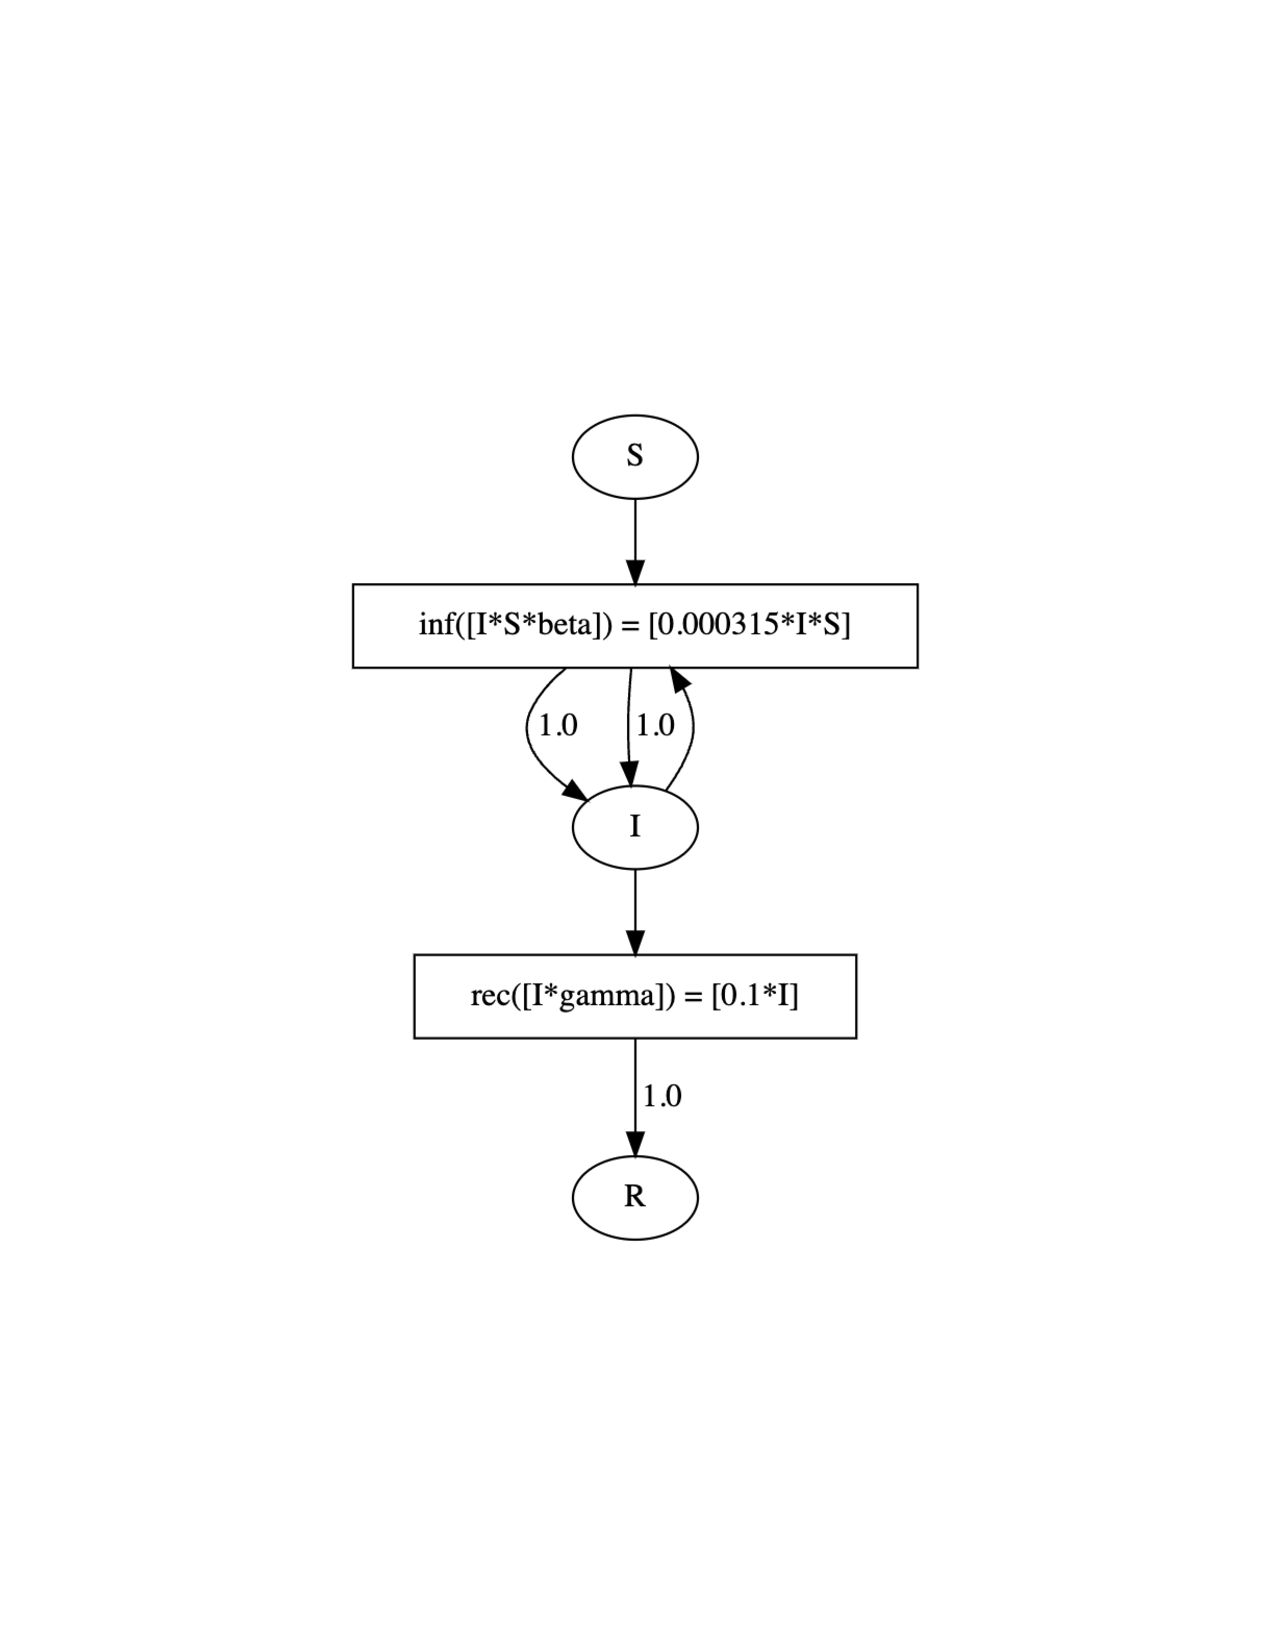
\includegraphics[width=0.3\linewidth,clip]{fig/sir/sir_model.pdf}
    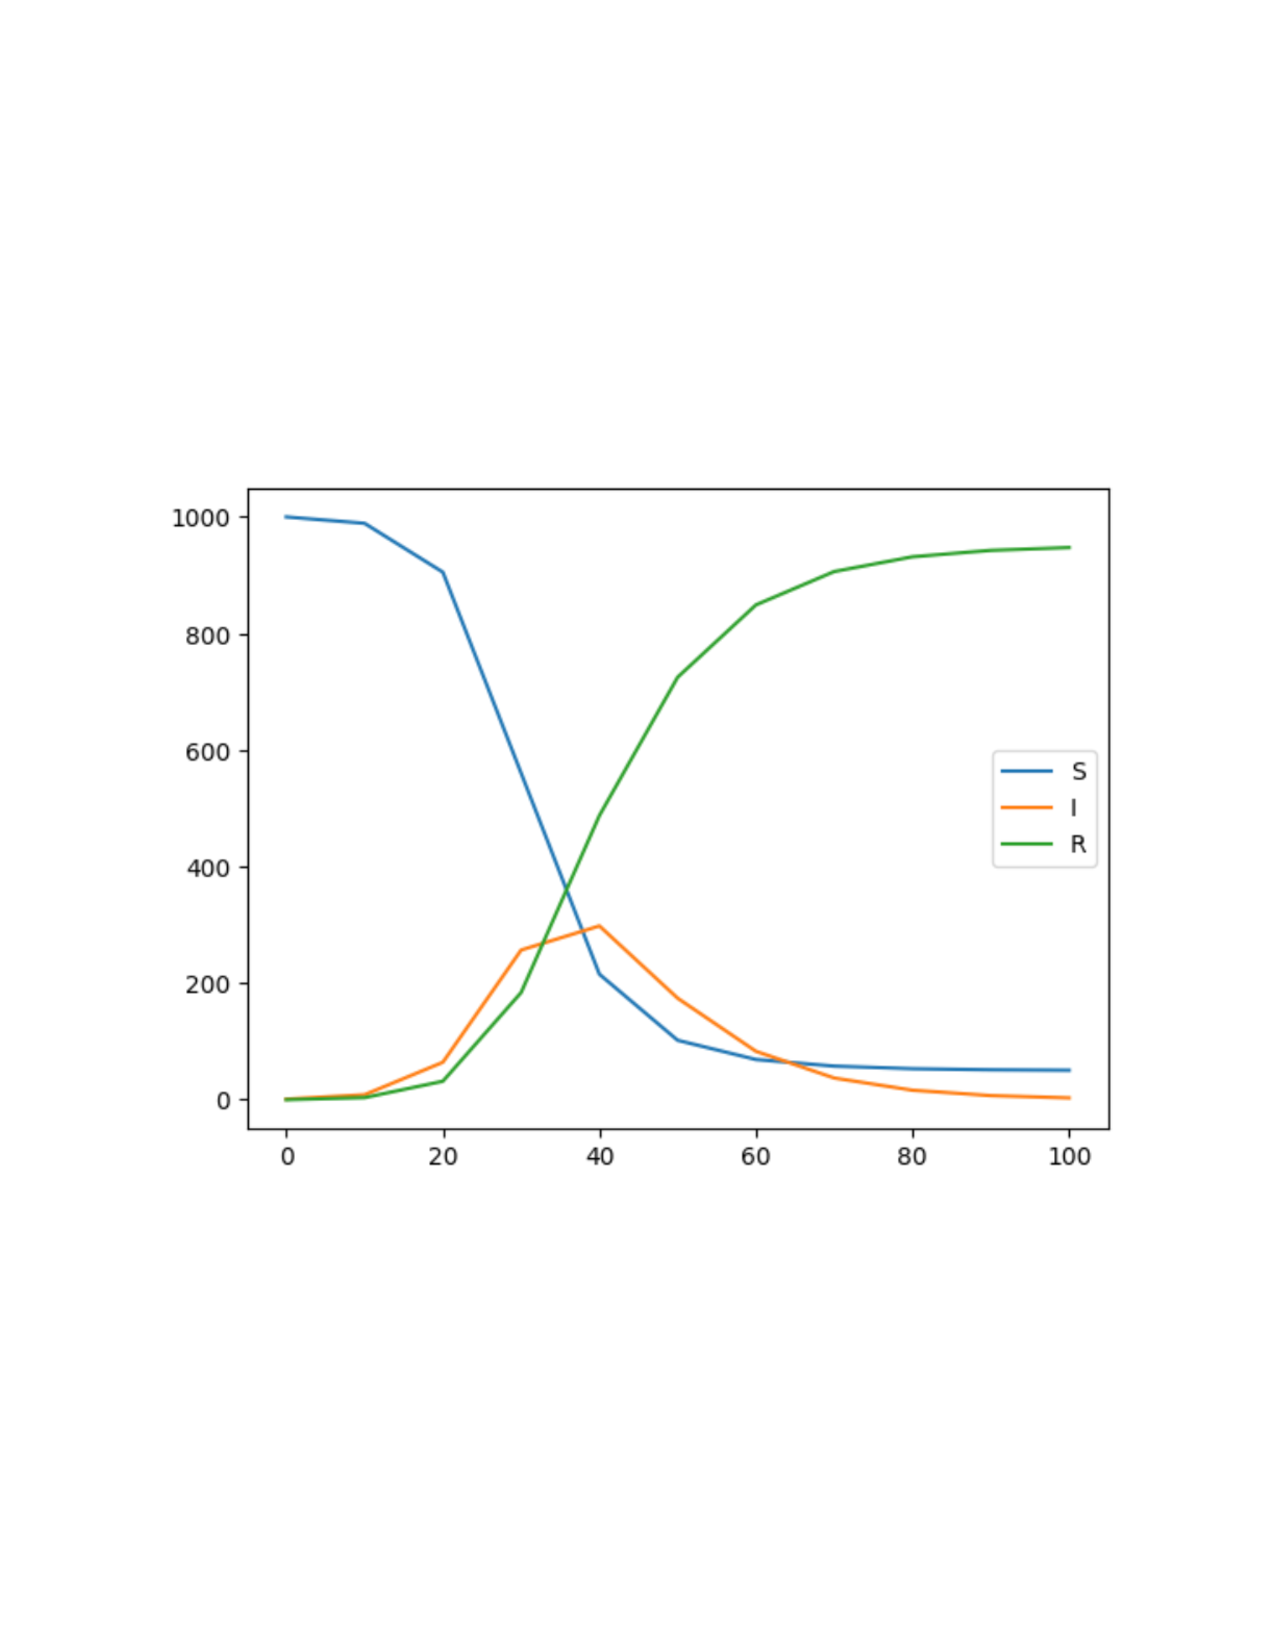
\includegraphics[width=0.4\linewidth,clip]{fig/sir/sir_sim.pdf}

    \caption{\label{fig:sir} Stratified SIR Model (left) and Simulation (right)}
\end{figure}

Figure \ref{fig:sir_bounded} illustrates the baseline SIR after transforming it to bound $S$, $I$, and $R$.  The corresponding lower and upper bounds for each state variable are denoted by a $\_lb$ or $\_ub$ suffix.  The model is different from the baseline in the following ways: there are six state variables and eight transitions, and the transitions use custom rates.  Each baseline transition is replaced by four transitions.  The four transitions differ in whether they define a lower or upper bound, and whether they define the flow into or out from a transition.  For example, the first transition `inf\_in\_lb' defines the lower bound on the flow from $S\_lb$ into the `inf' transition.  The least flow expression is illustrated in the box for the transition.  Simulating this model with the same initial state and parameters (where the lower and upper bounds are initially equal) results in a simulation where the lower and upper bounds are equal for all variables.  While bounding this model in this fashion is not useful in itself, it illustrates a simple application of the bounding transformation.  The bounded abstraction, described below, is similar except that it uses alternative bounds on the parameters.  

\begin{figure}[t]
    \centering
    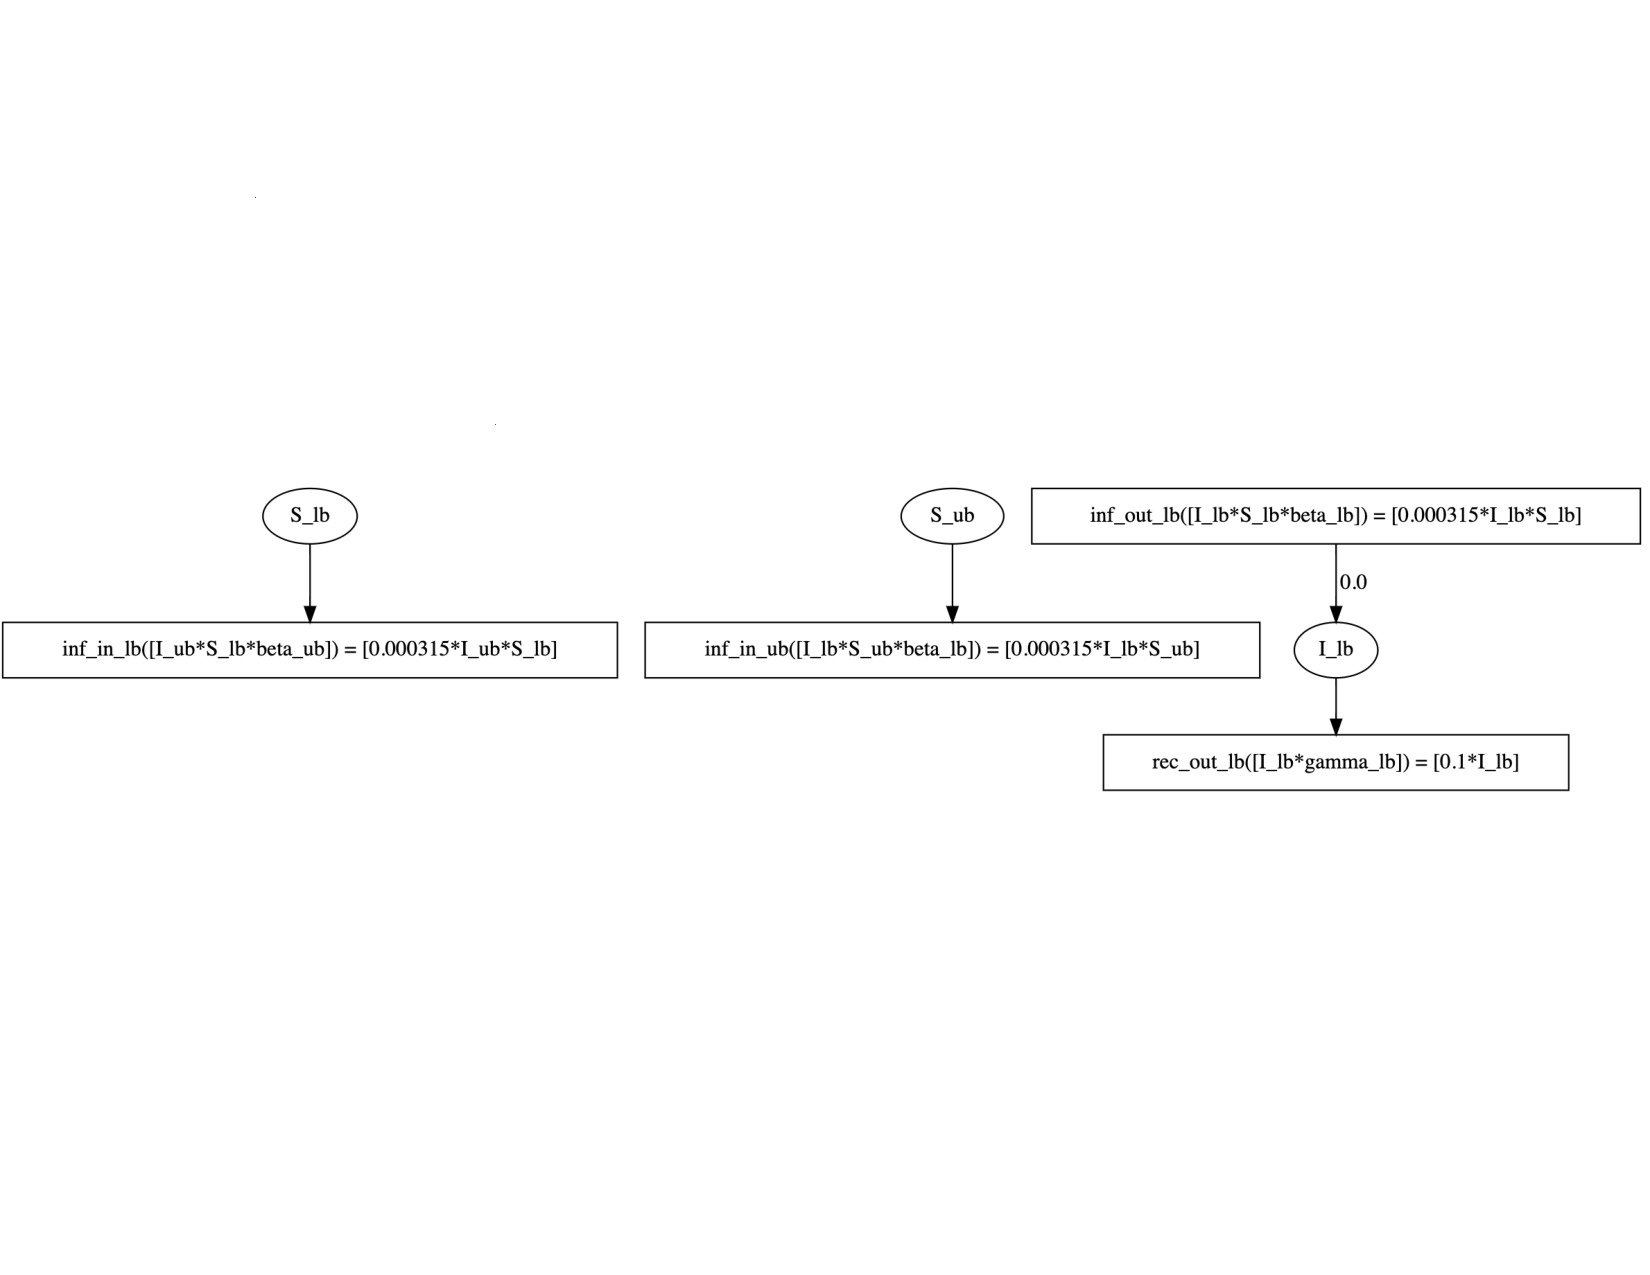
\includegraphics[width=0.8\linewidth,clip,trim={0 8cm 0 8cm}]{fig/sir/sir_bounded_model_1.pdf}
    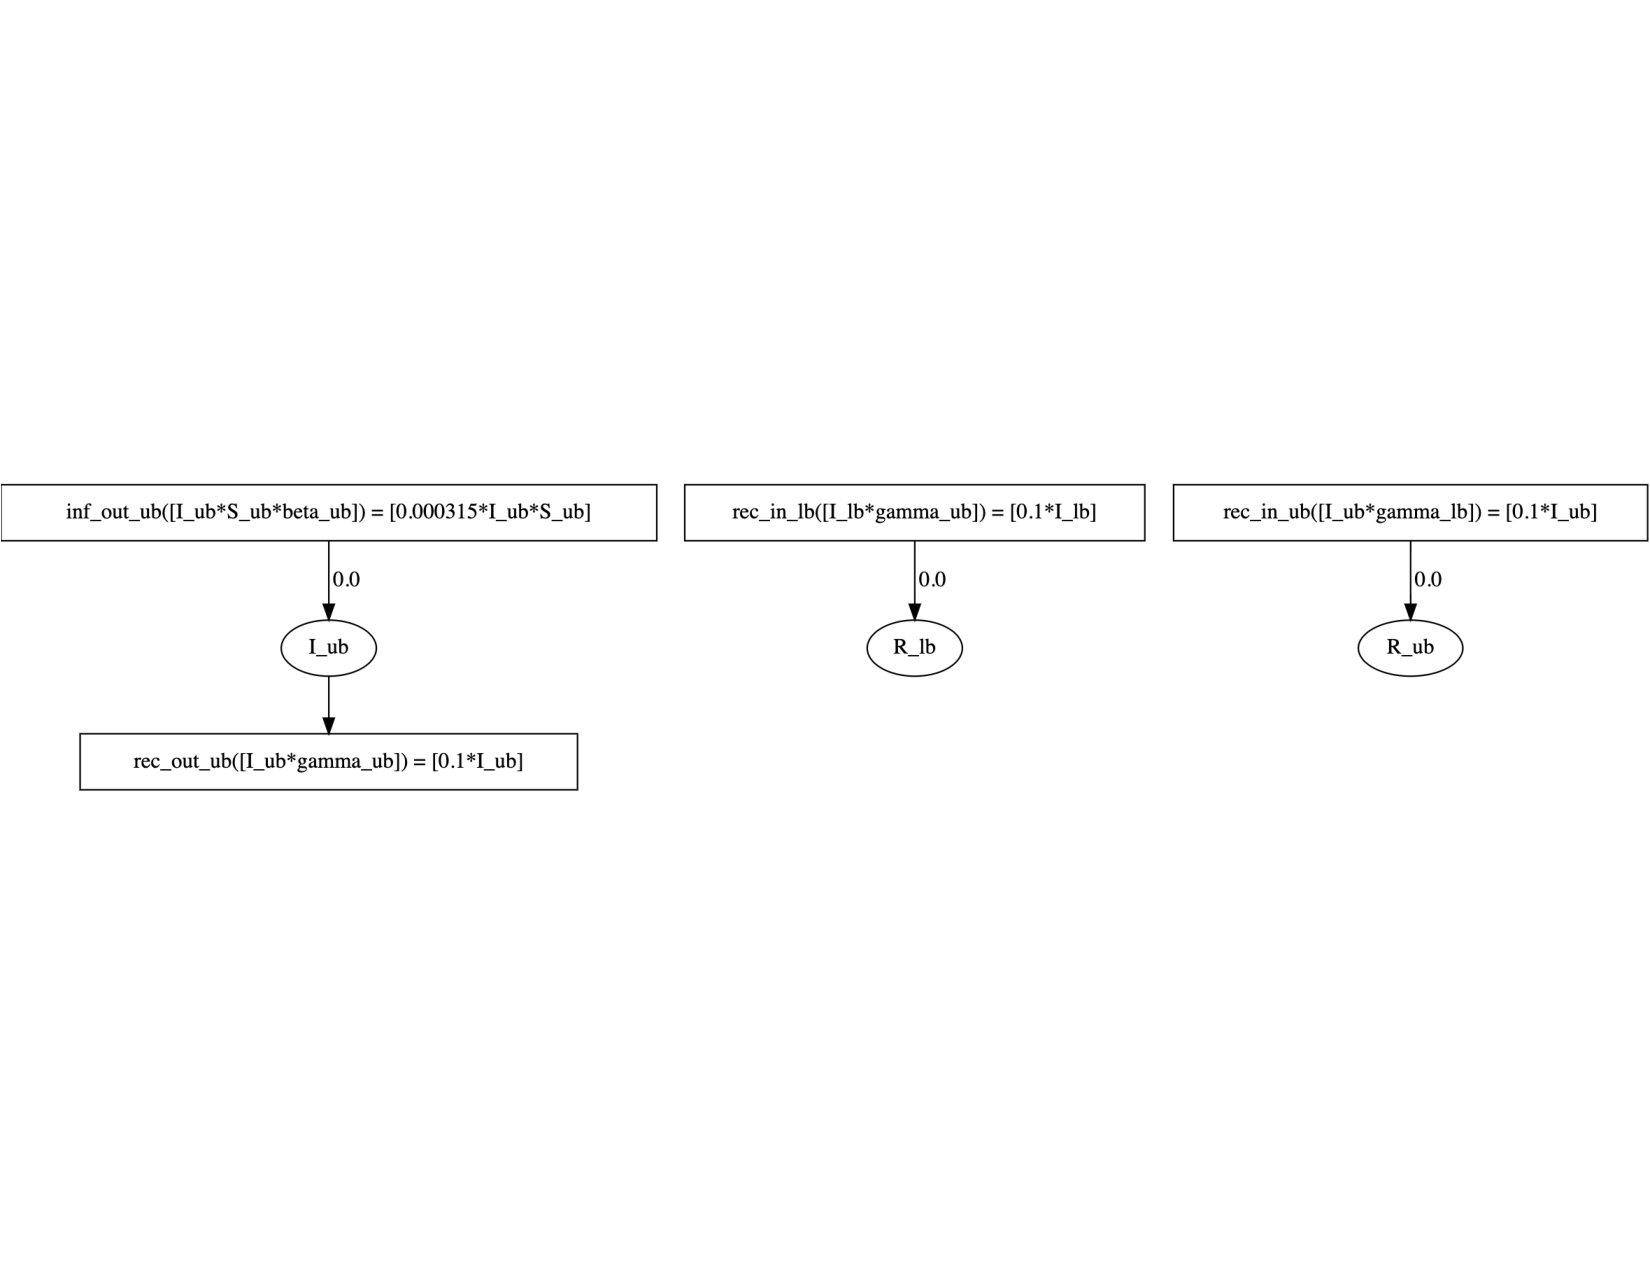
\includegraphics[width=0.8\linewidth,clip]{fig/sir/sir_bounded_model_2.pdf}
    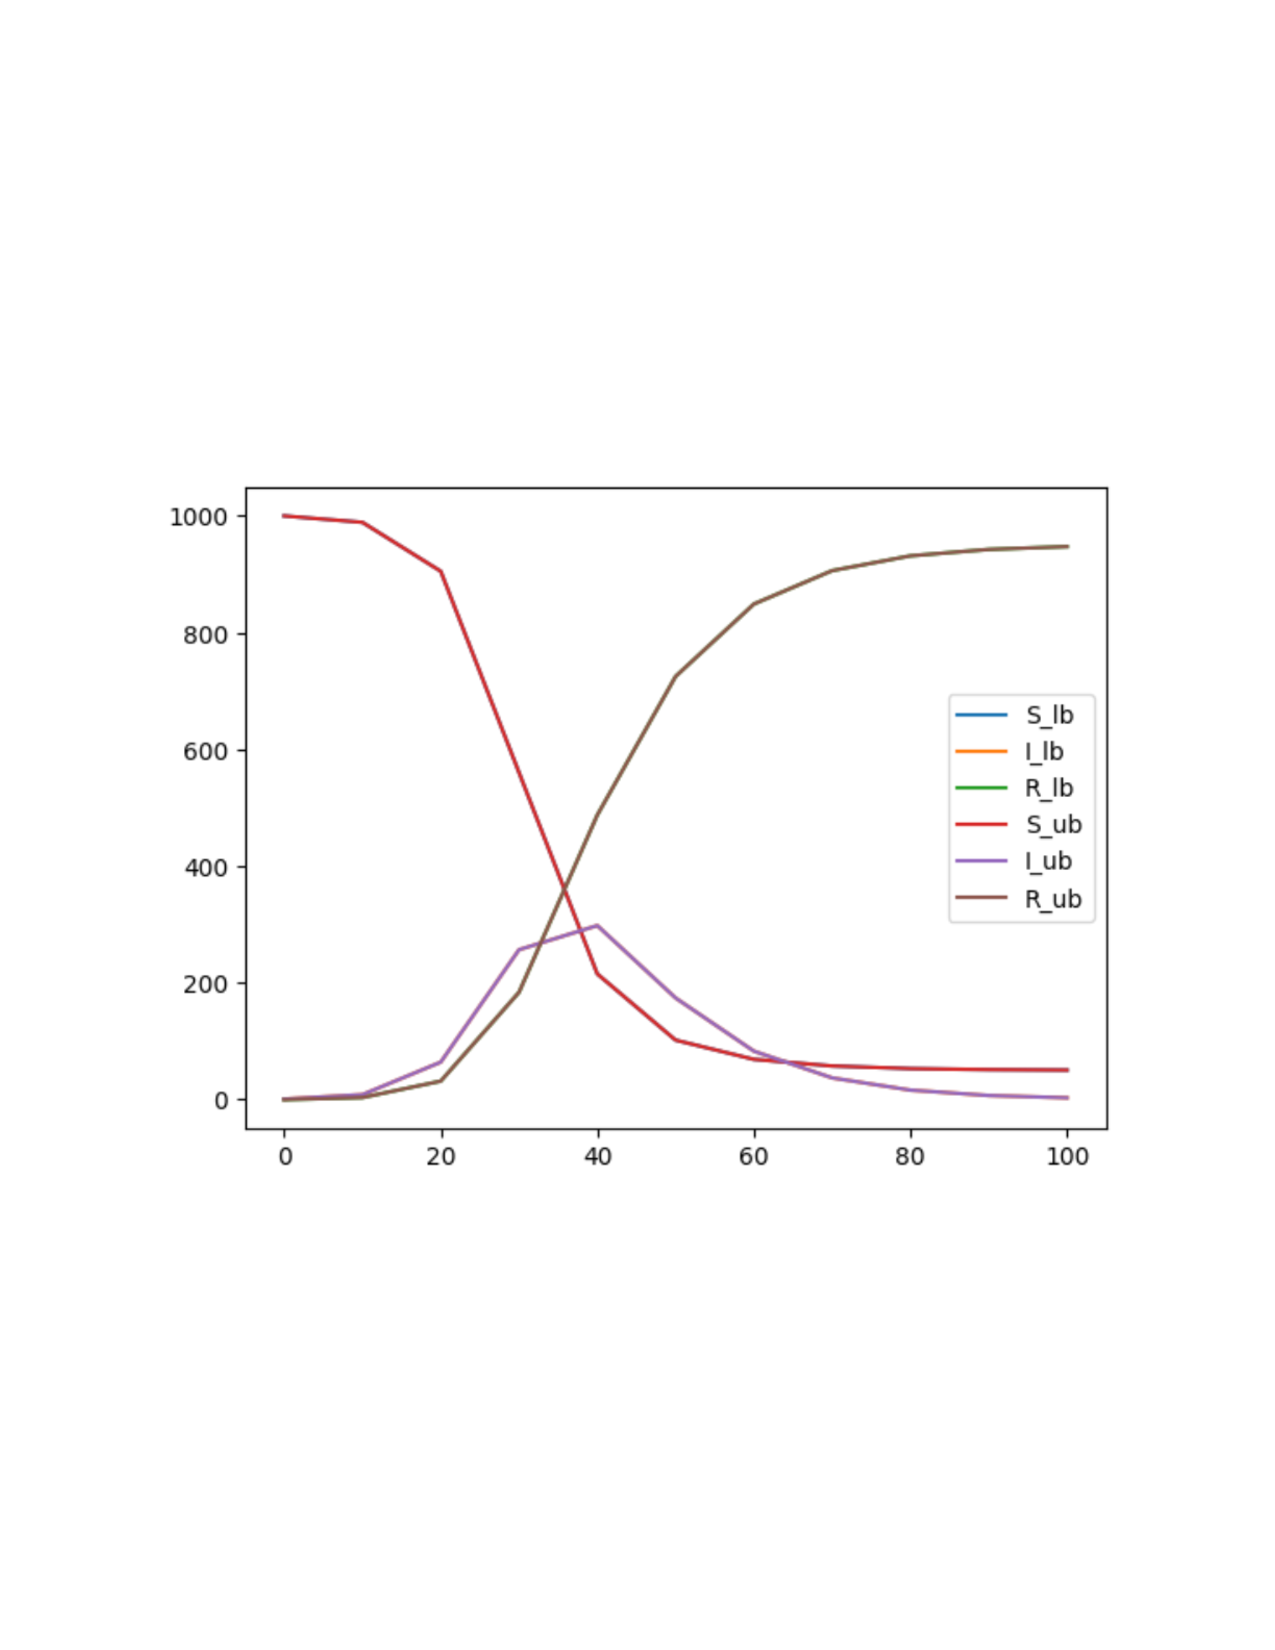
\includegraphics[width=0.4\textwidth,clip]{fig/sir/sir_bounded_sim.pdf}
    \caption{\label{fig:sir_bounded} Bounded SIR Model (top) and Simulation (bottom)}
\end{figure}

Figure \ref{fig:sir_stratified} illustrates the stratified SIR model (wrt. $S$).  It uses state variables that distinguish two $S$ populations and two $inf$ transitions that distinguish different rates due to two $\beta$ parameters.  We modified the $\beta$ parameters to be slightly less and greater than $\beta$ from the previous models.  The simulation illustrates a difference between the $S$ variables.

\begin{figure}[t]
    \centering
    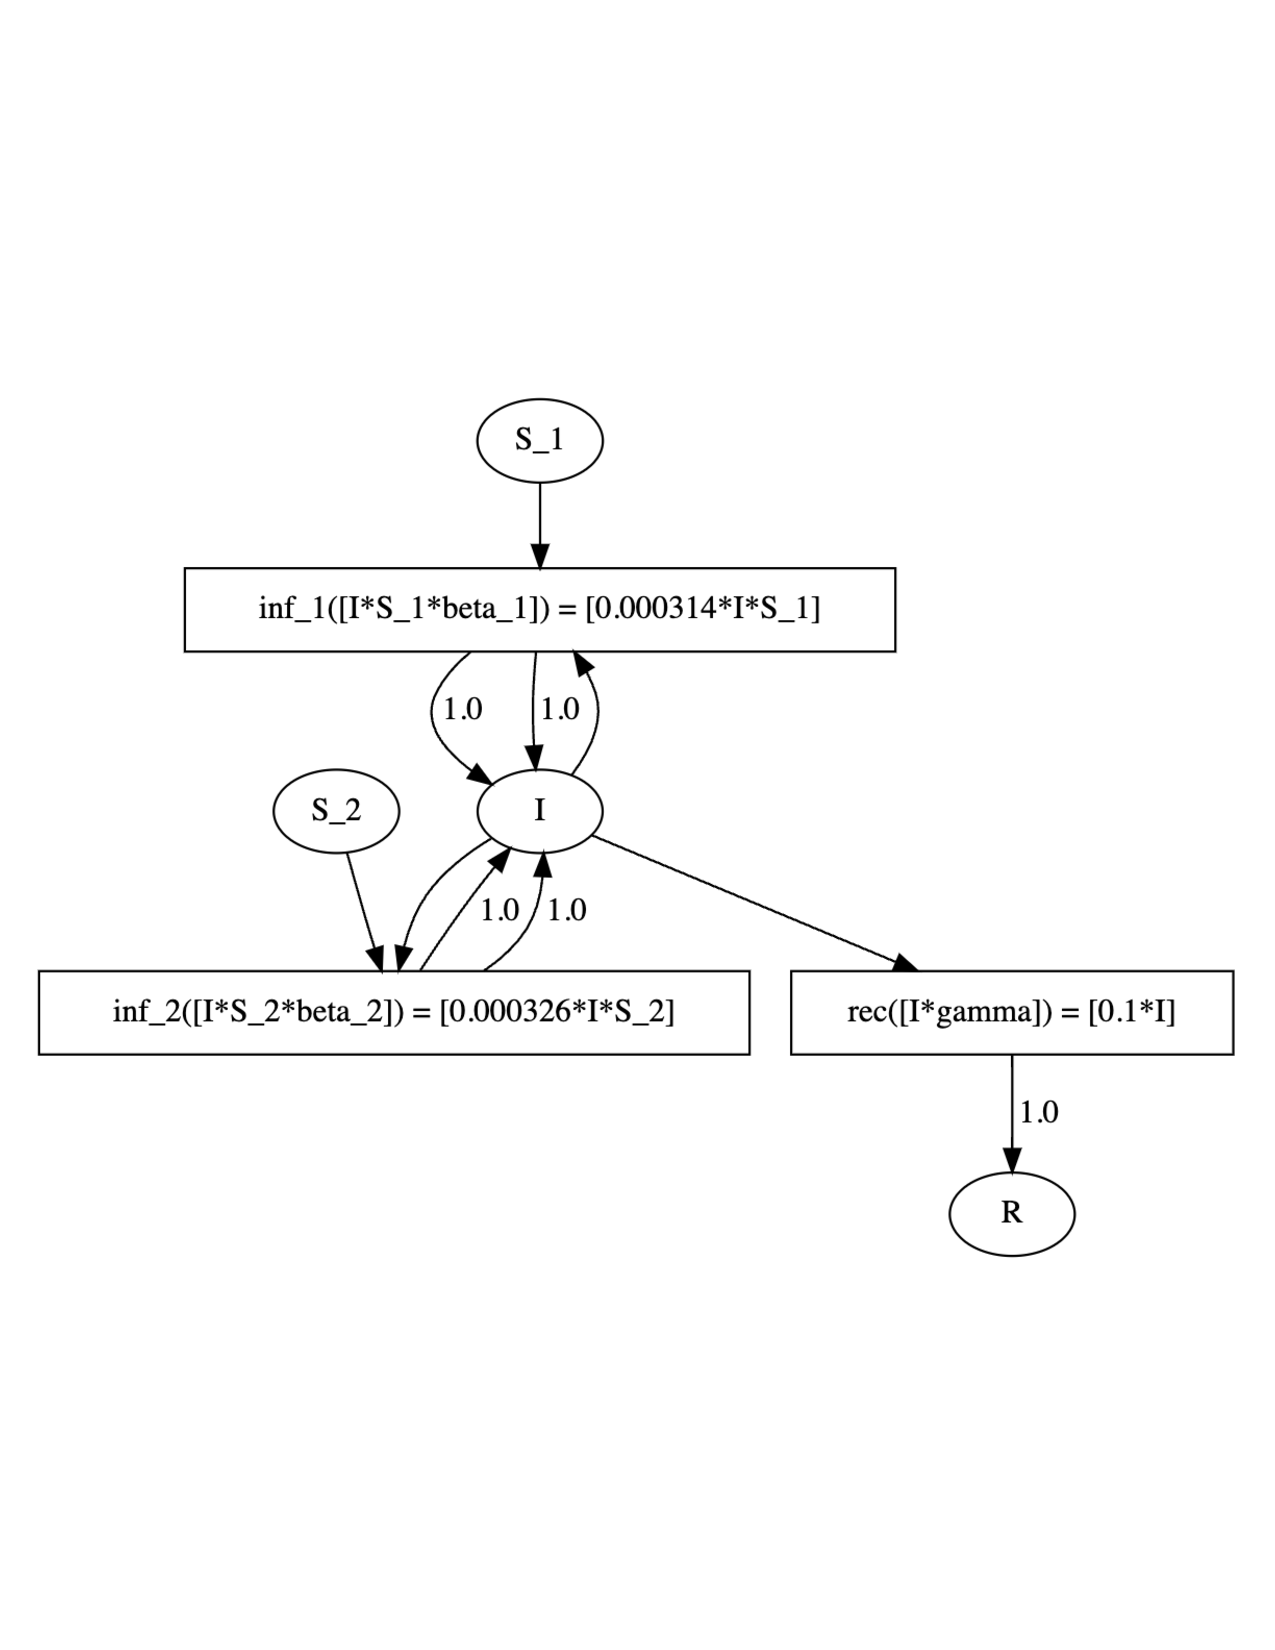
\includegraphics[width=0.5\linewidth,clip]{fig/sir/sir_stratified_model.pdf}
    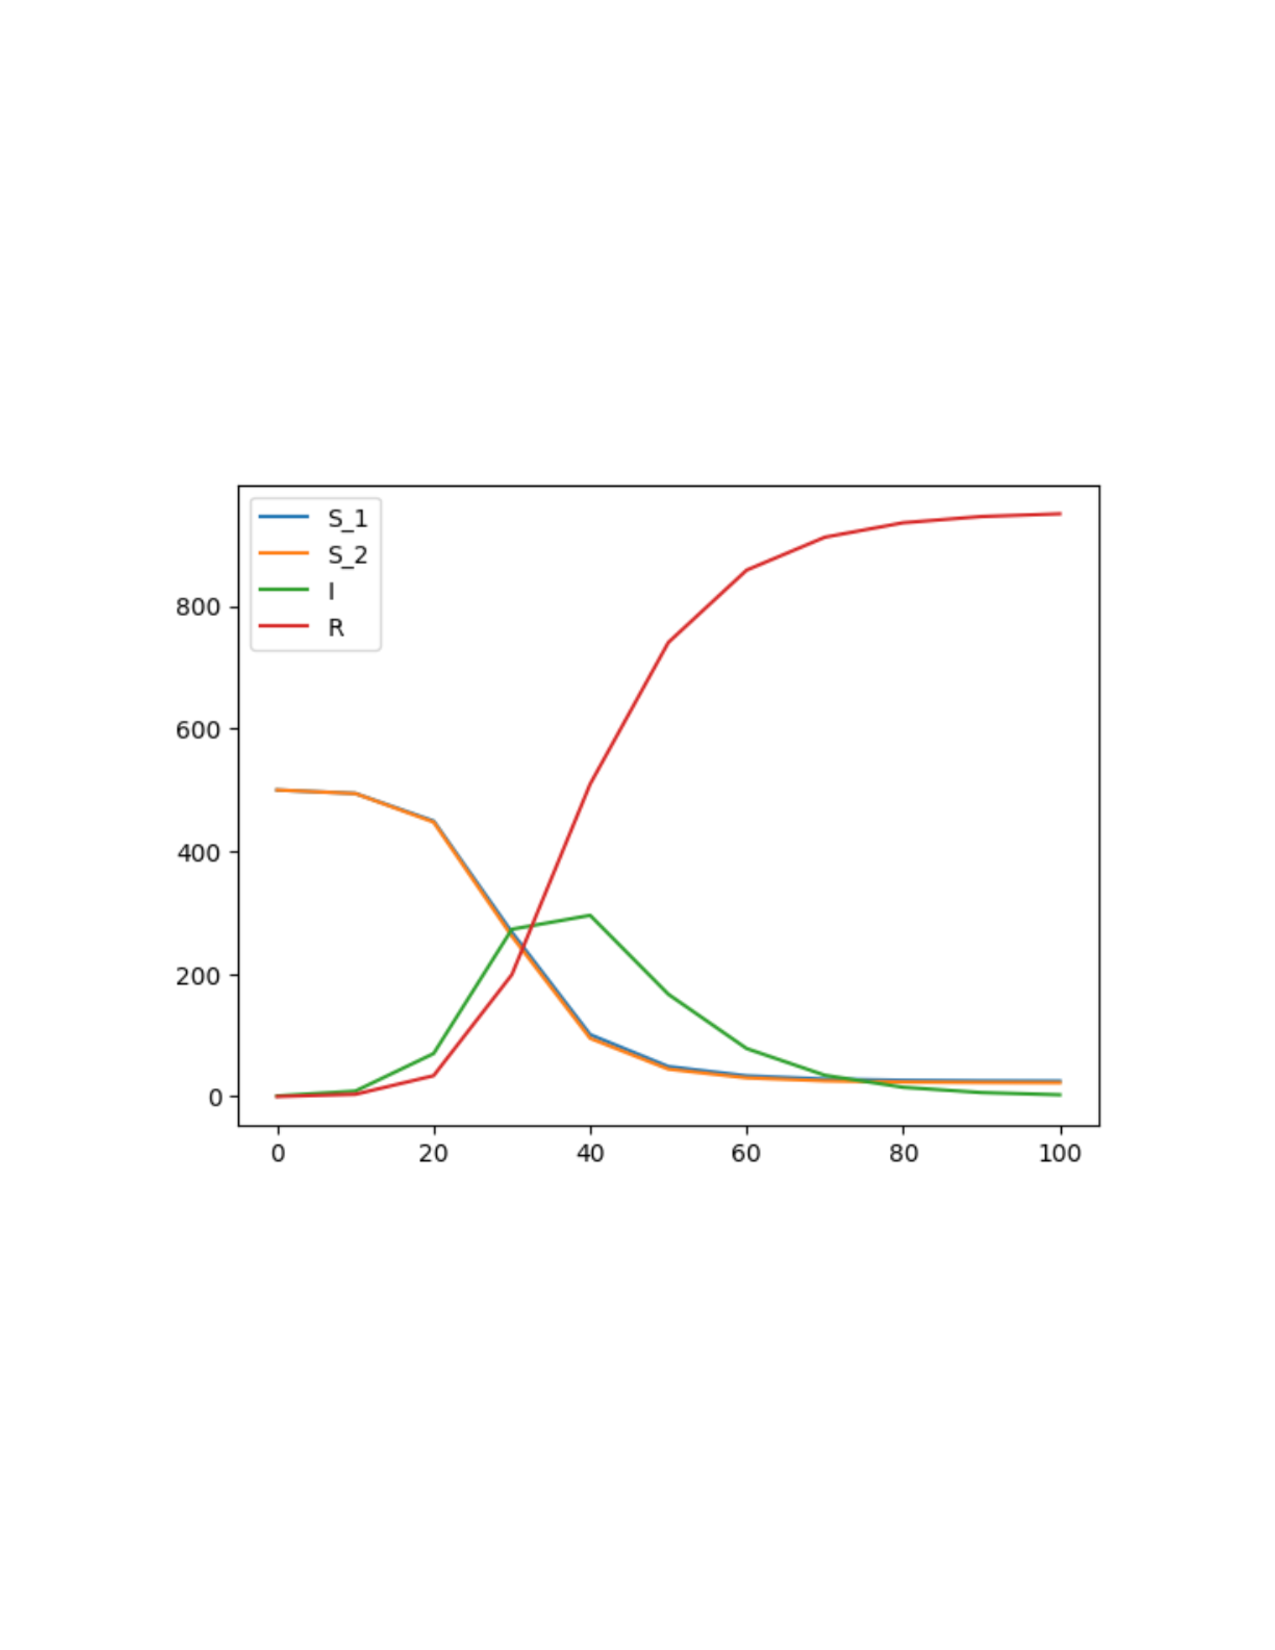
\includegraphics[width=0.4\linewidth,clip]{fig/sir/sir_stratified_sim.pdf}
    \caption{\label{fig:sir_stratified} Stratified SIR Model (top) and Simulation (bottom)}
\end{figure}

Figure \ref{fig:sir_bounded_stratified} illustrates a bounded stratified model, for the sake of illustration.  It resembles the bounded baseline model aside from incorporating the stratified $S$ variable.  The simulation shows how it is possible to bound the stratified variables and achieve similar results to prior models. The primary distinction with this model is how it bounds the stratified variables individually instead of collectively.  The collective bounding can be achieved by first abstracting and then bounding the stratified variables.

\begin{figure}[t]
    \centering
    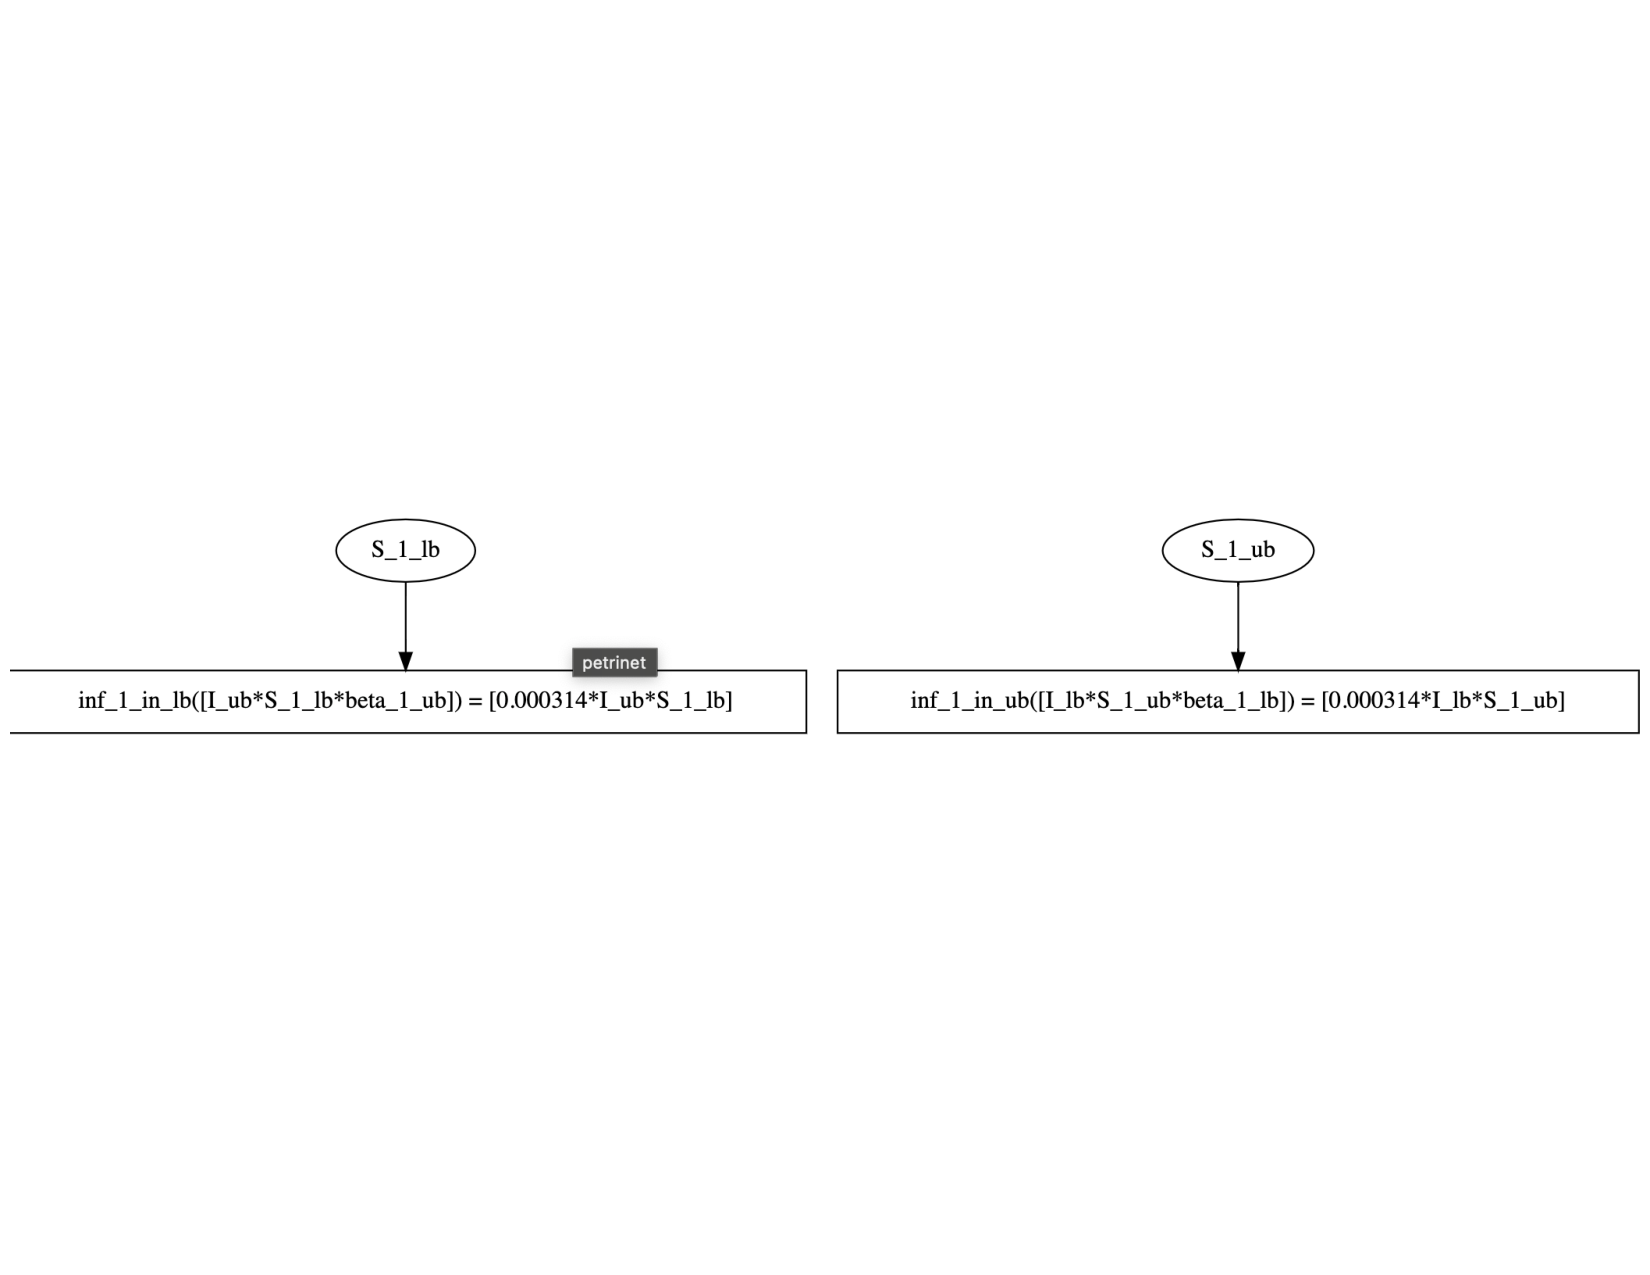
\includegraphics[width=0.6\linewidth,clip]{fig/sir/sir_bounded_stratified_1.pdf}
    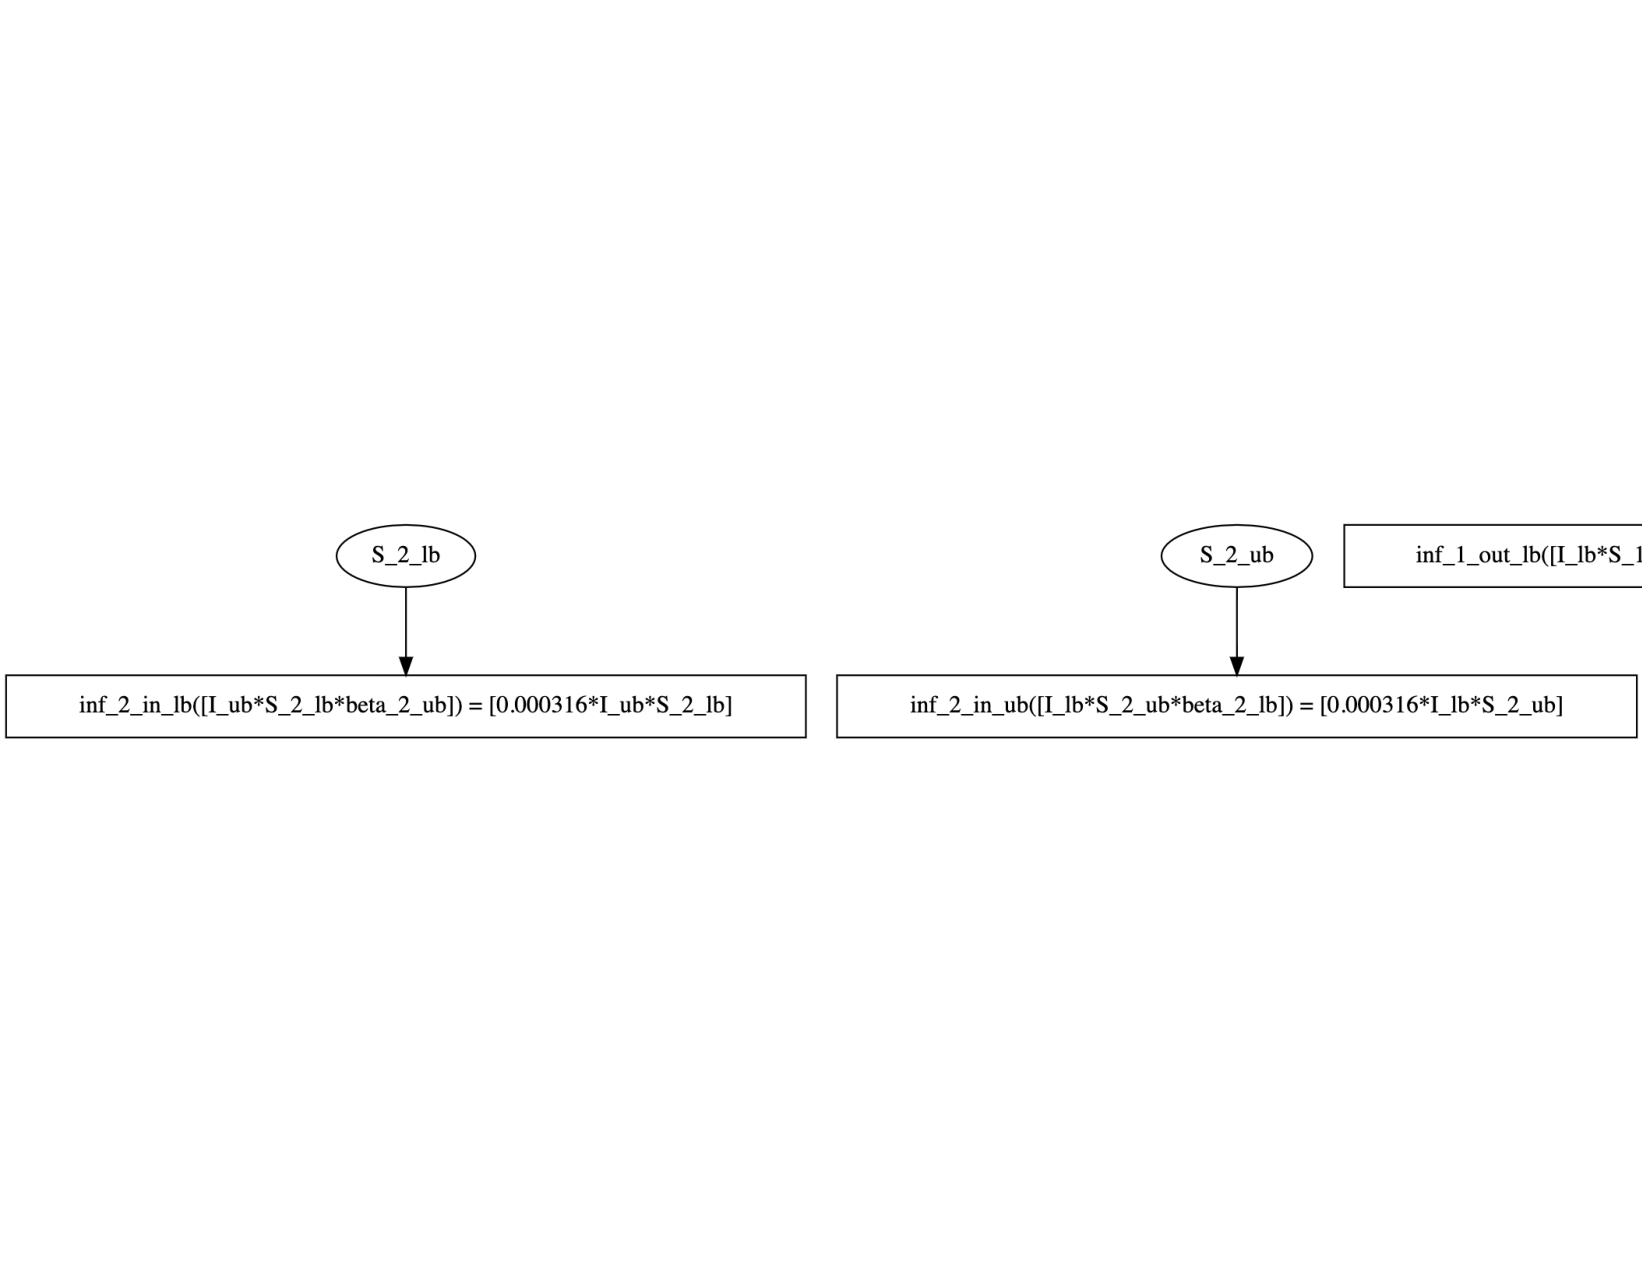
\includegraphics[width=0.6\linewidth,clip]{fig/sir/sir_bounded_stratified_2.pdf}
    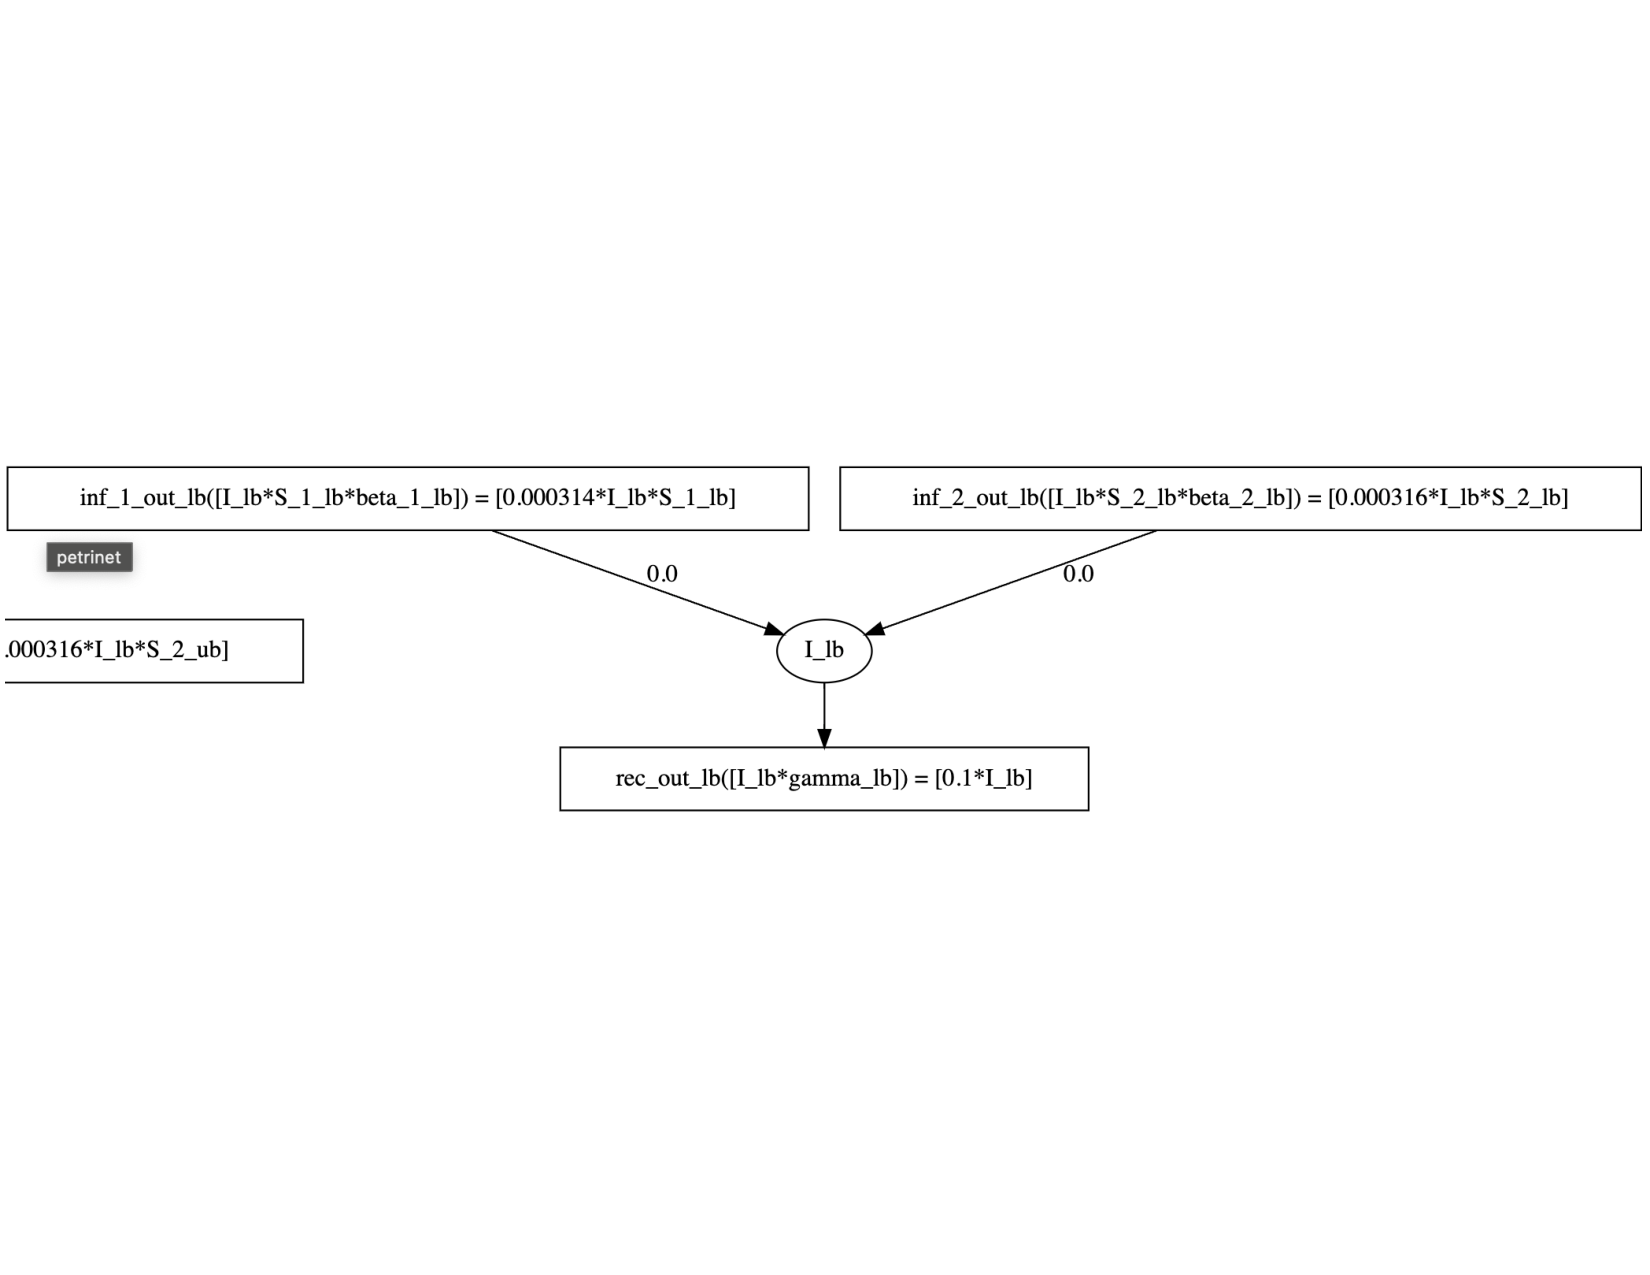
\includegraphics[width=0.6\linewidth,clip]{fig/sir/sir_bounded_stratified_3.pdf}
    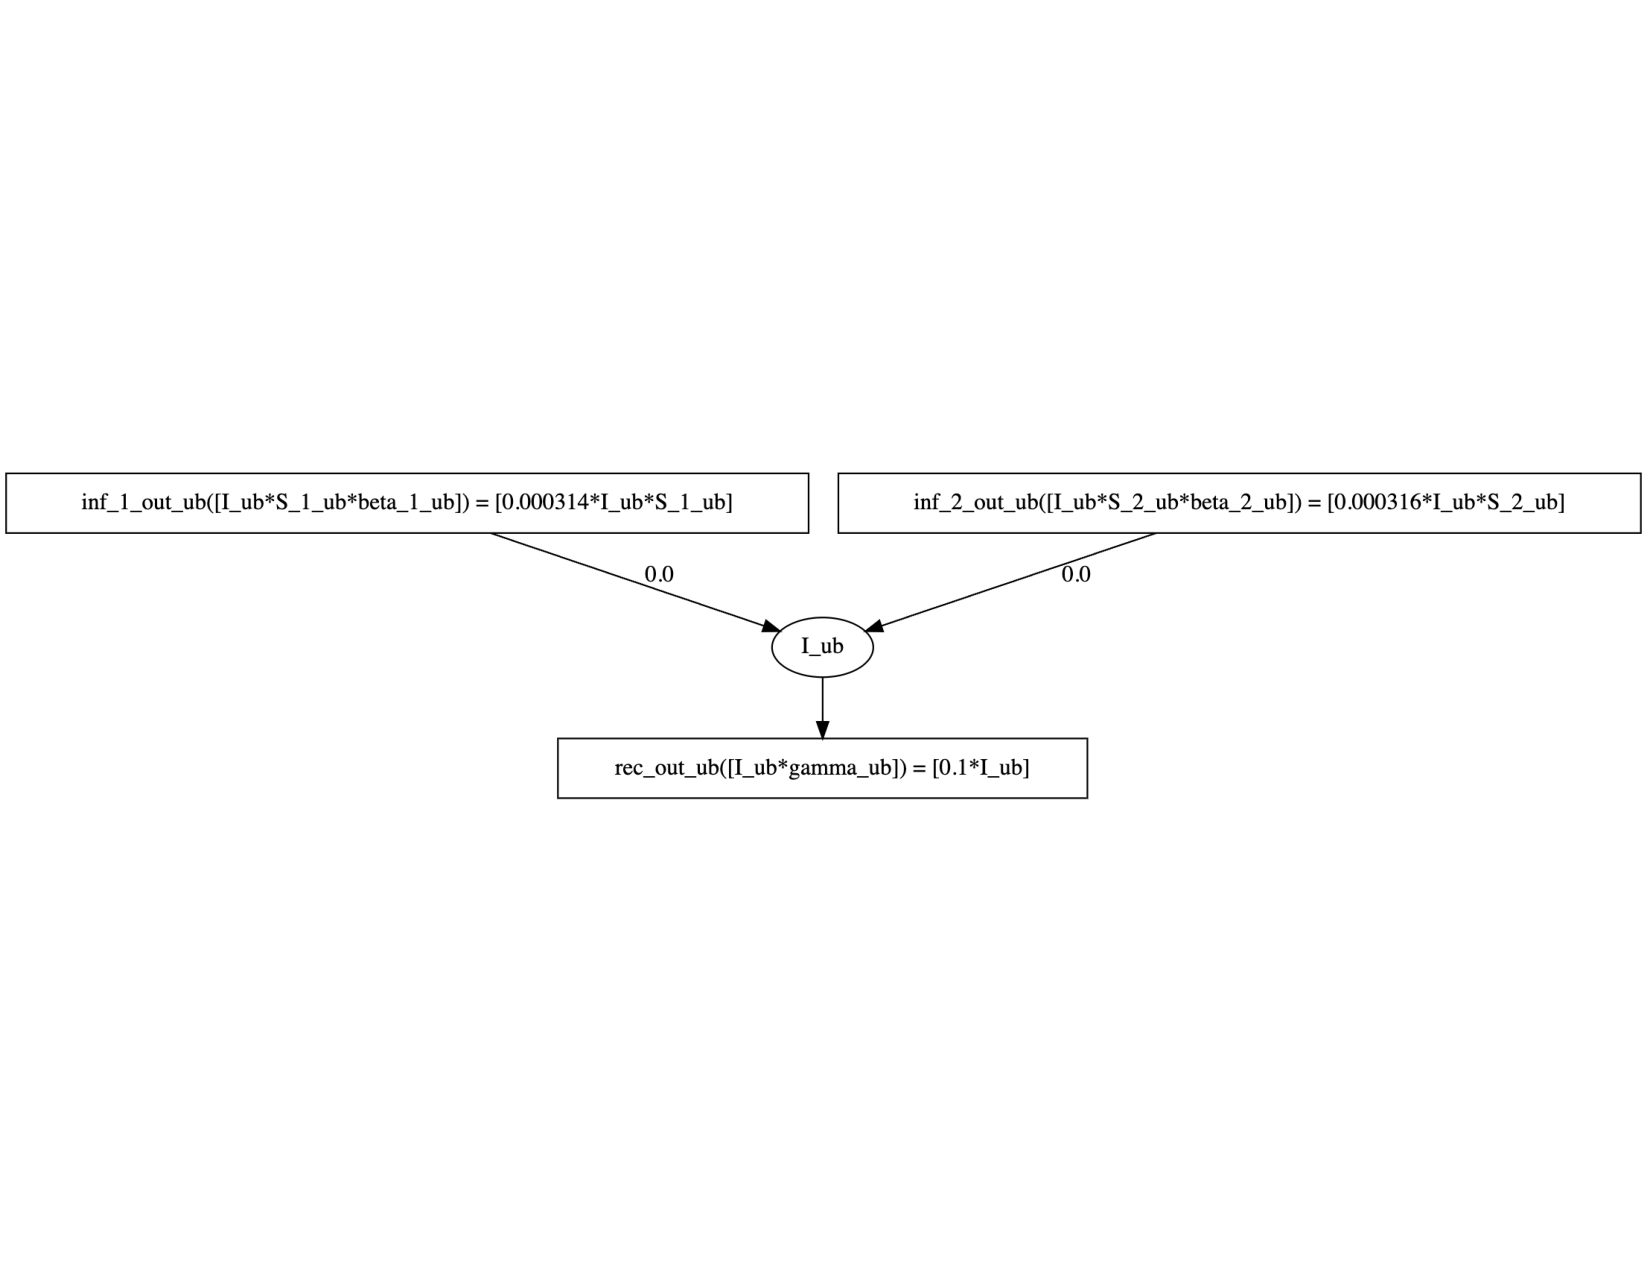
\includegraphics[width=0.6\linewidth,clip]{fig/sir/sir_bounded_stratified_4.pdf}
    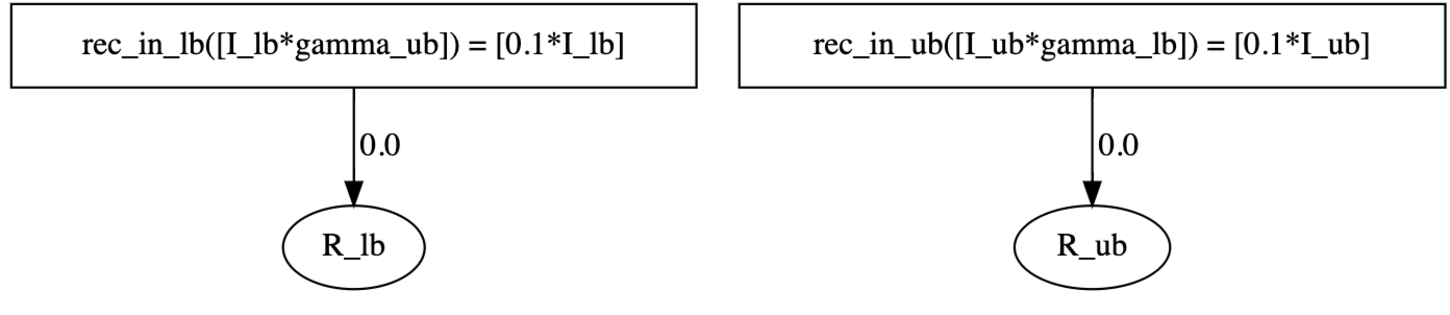
\includegraphics[width=0.4\linewidth,clip]{fig/sir/sir_bounded_stratified_5.pdf}\\
    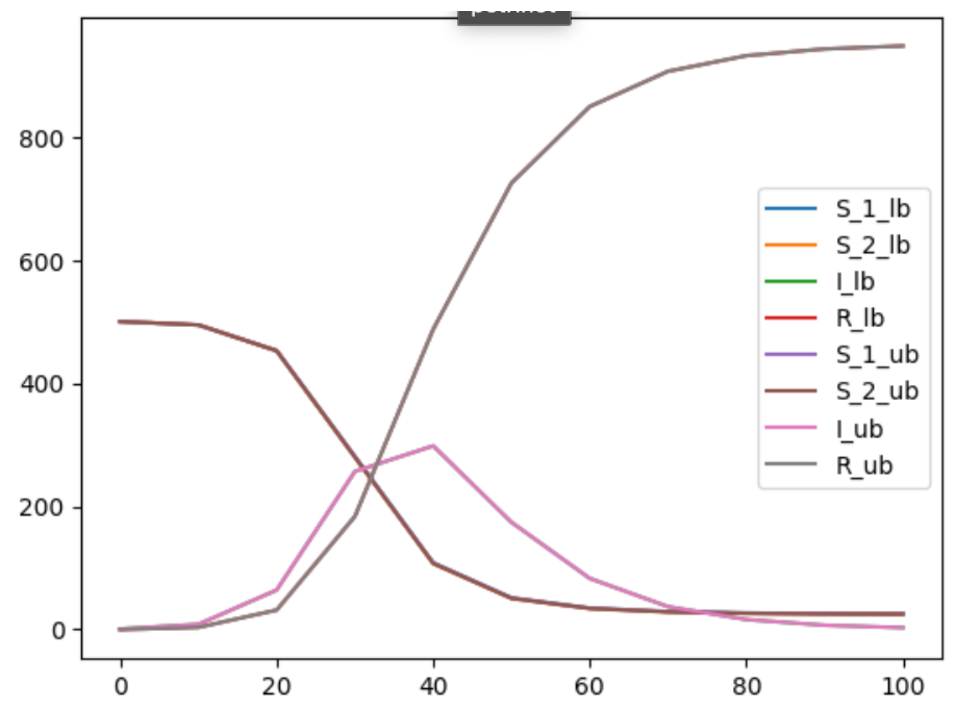
\includegraphics[width=0.4\linewidth,clip]{fig/sir/sir_bounded_stratified_sim.pdf}
    \caption{\label{fig:sir_bounded_stratified} Bounded Stratified SIR Model (top) and Simulation (bottom)}
\end{figure}


Figure \ref{fig:sir_abstract_bounded_stratified}  illustrates the bounded abstracted model.  It resembles the bounded baseline model, except that it incorporates upper and lower bounds on the $\beta$ parameter due to the stratified populations.  By propagating lower and upper bounds that are not equal, this variation of the model captures lower and upper bounds on the abstracted state variables.  The bounds are tight enough to answer several queries about the model.  For example, it can assess whether a upper threshold (that does not fall between the bounds) on peak infected $I$ is satisfied.  The threshold $I \leq 400$ is satisfied because $I\_ub \leq 400$.  However, the threshold $I \leq 300$ may or may not be satisfied because $I\_lb \leq 300 \leq I\_ub$.

\begin{figure}[t]
    \centering
    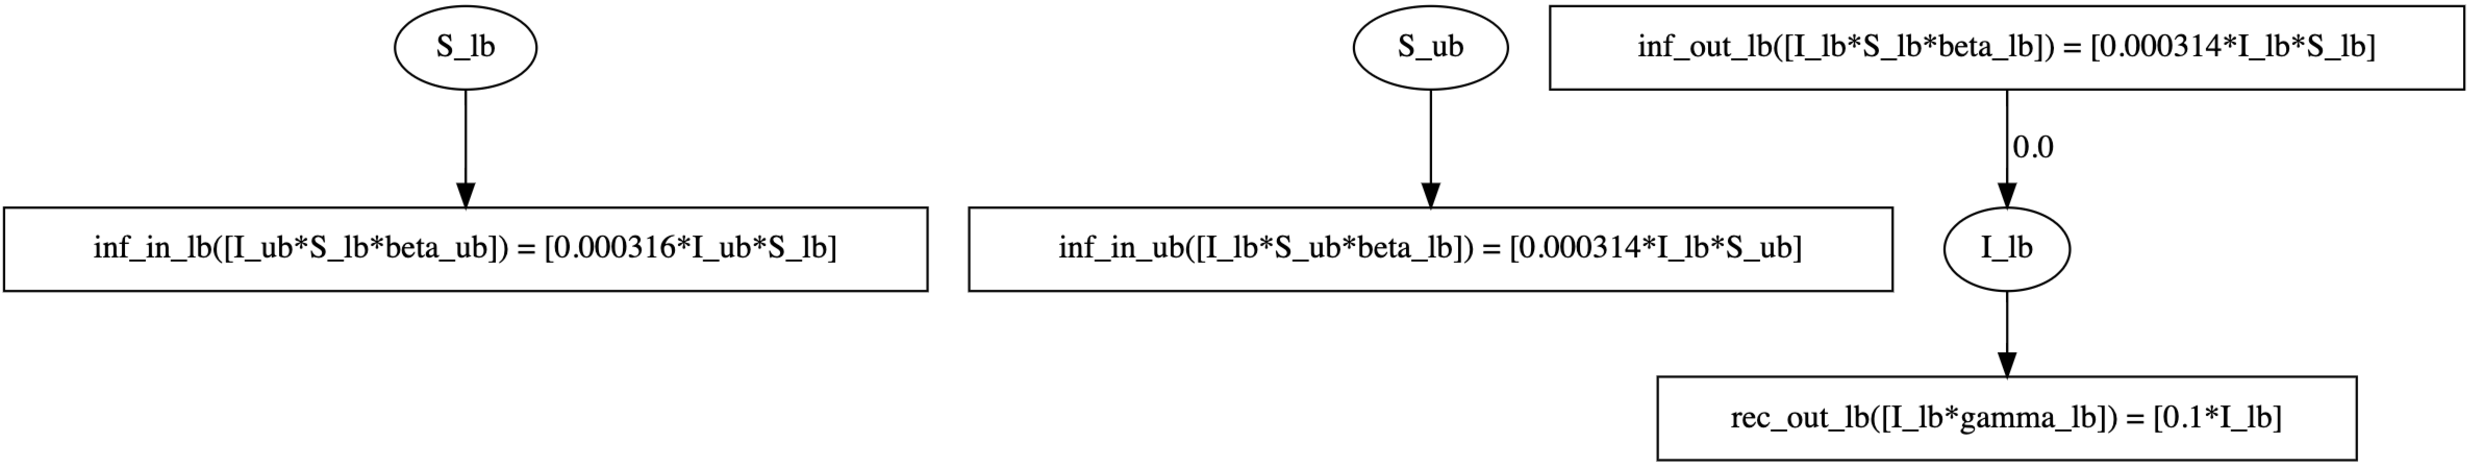
\includegraphics[width=0.6\linewidth,clip]{fig/sir/sir_abstract_bounded_model_1.pdf}
    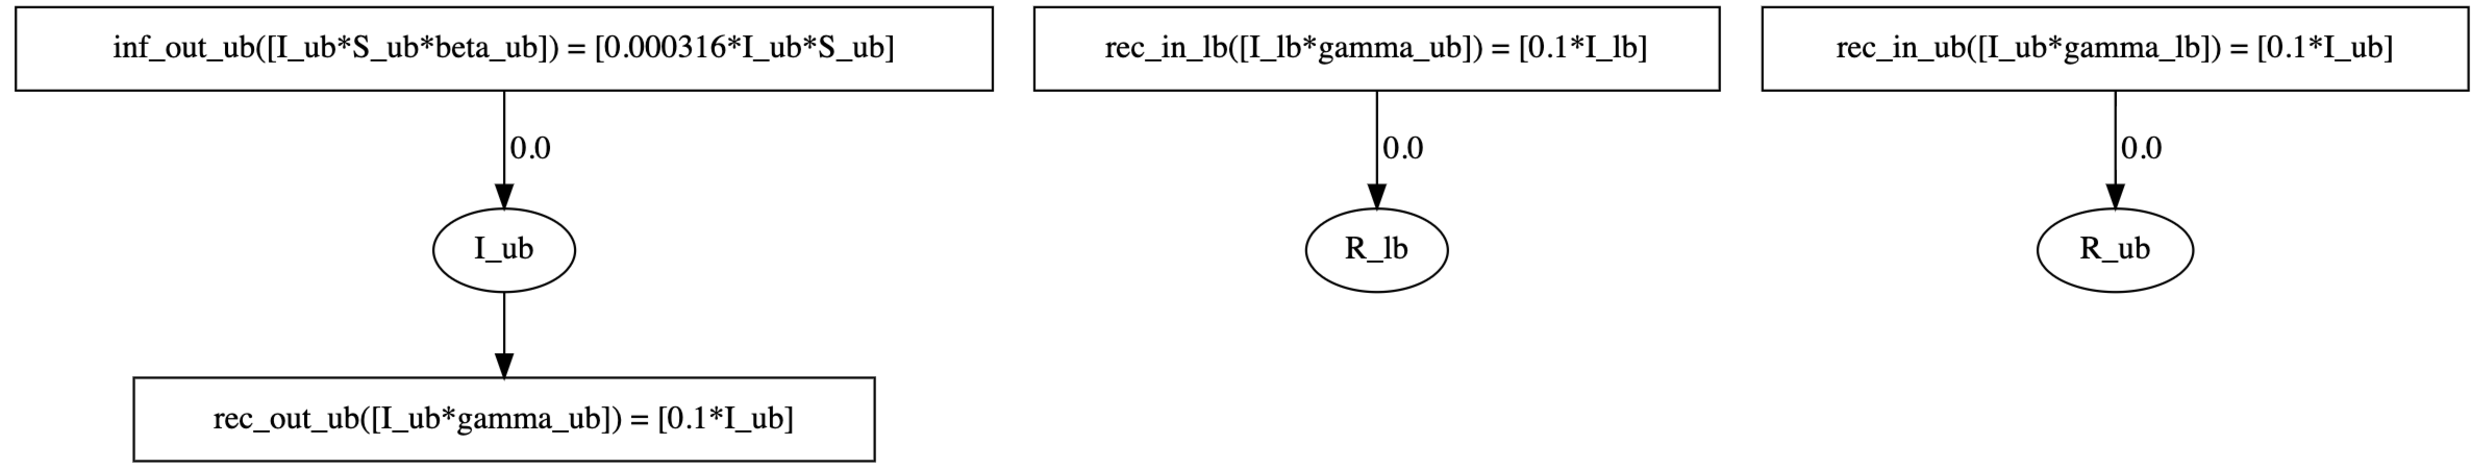
\includegraphics[width=0.6\linewidth,clip]{fig/sir/sir_abstract_bounded_model_2.pdf}
    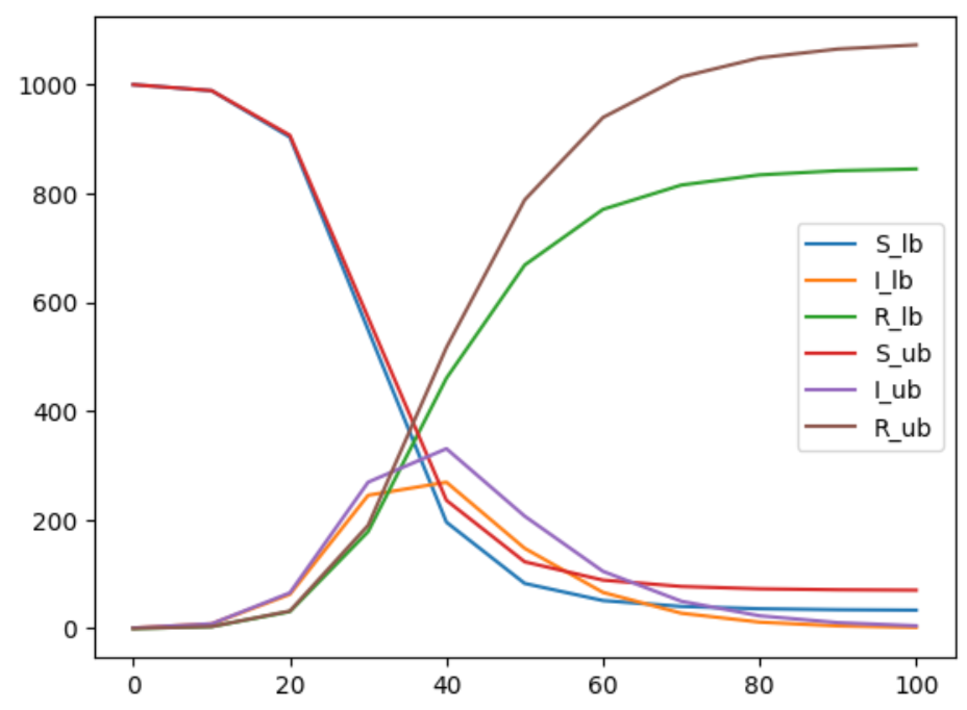
\includegraphics[width=0.4\linewidth,clip]{fig/sir/sir_abstract_bounded_sim.pdf}
    \caption{\label{fig:sir_abstract_bounded_stratified} Bounded Stratified SIR Model (top) and Simulation (bottom)}
\end{figure}

% \begin{figure}
%     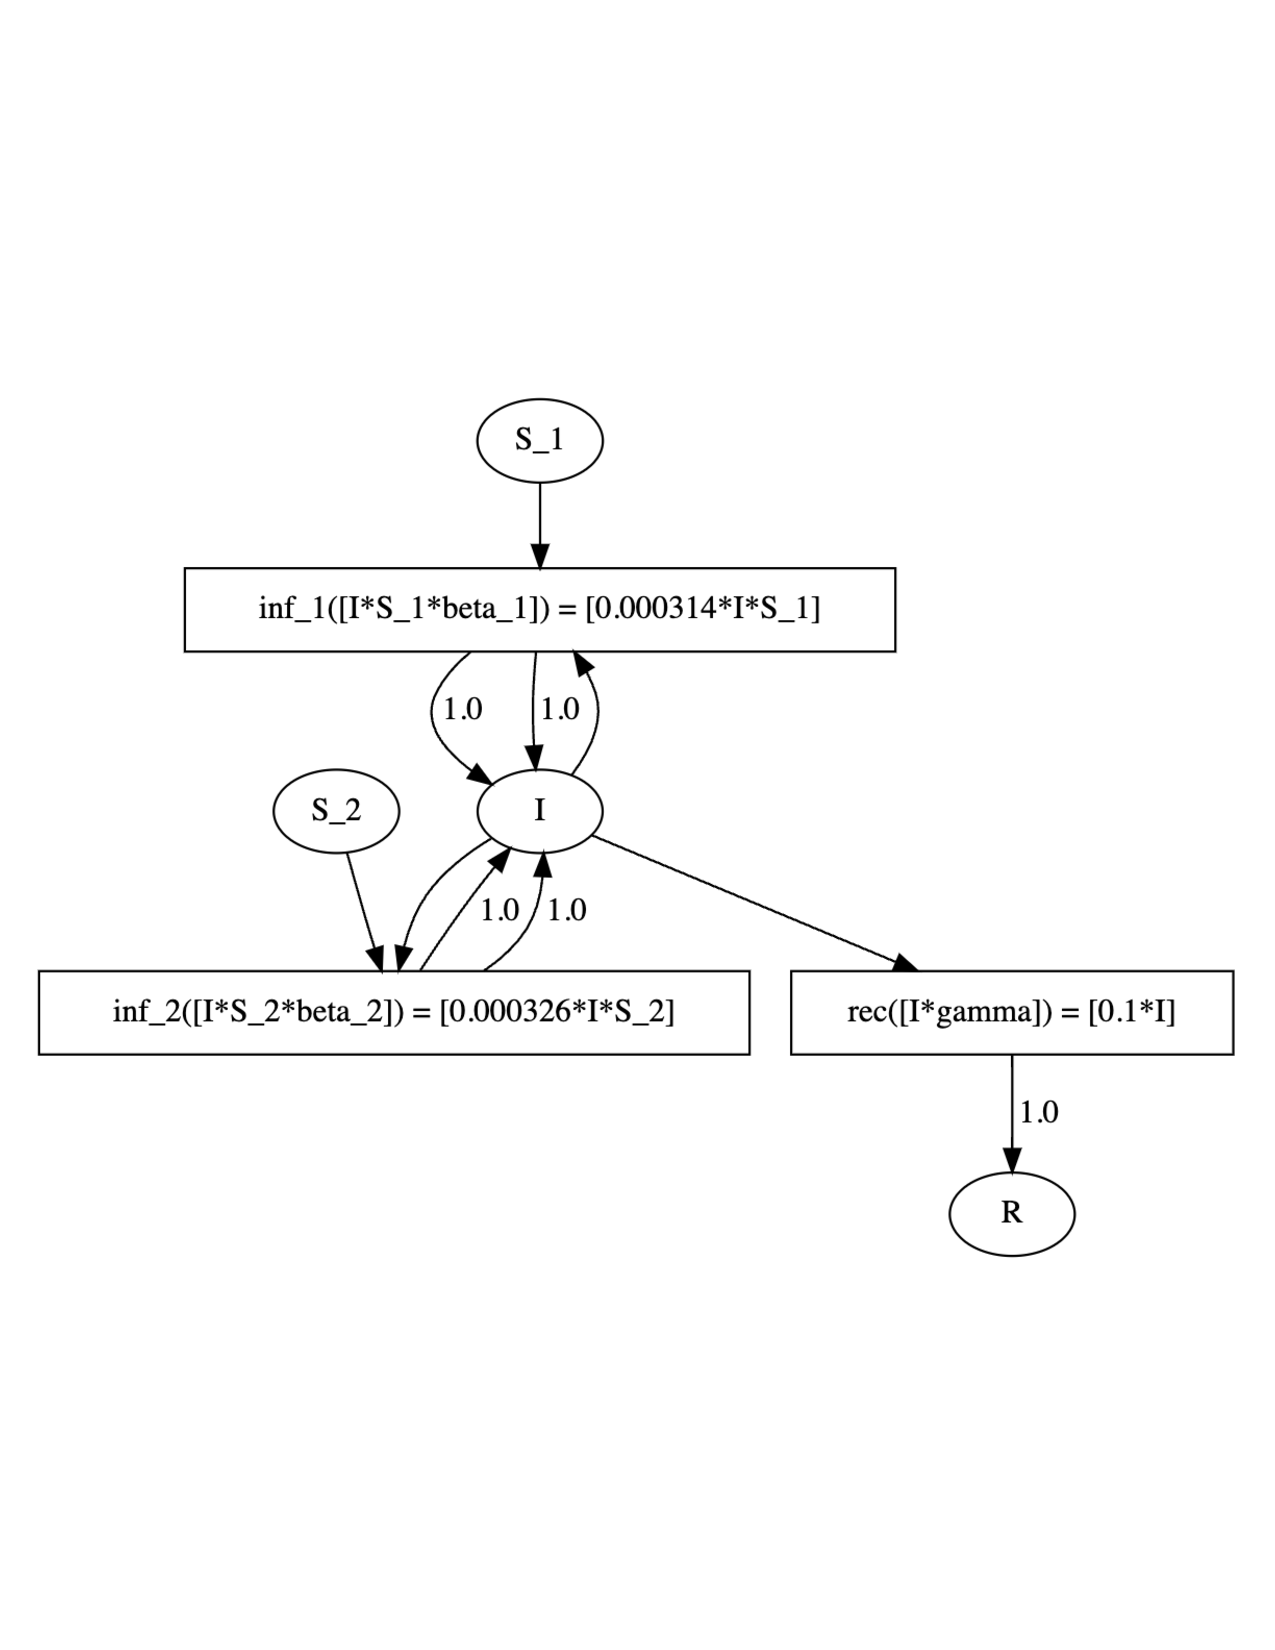
\includegraphics[width=\linewidth]{fig/sir/sir_stratified_model.pdf}
% %     \caption{\label{fig:sir_stratified_model} Stratified SIR Model}
% % \end{figure}

% % \begin{figure}
%     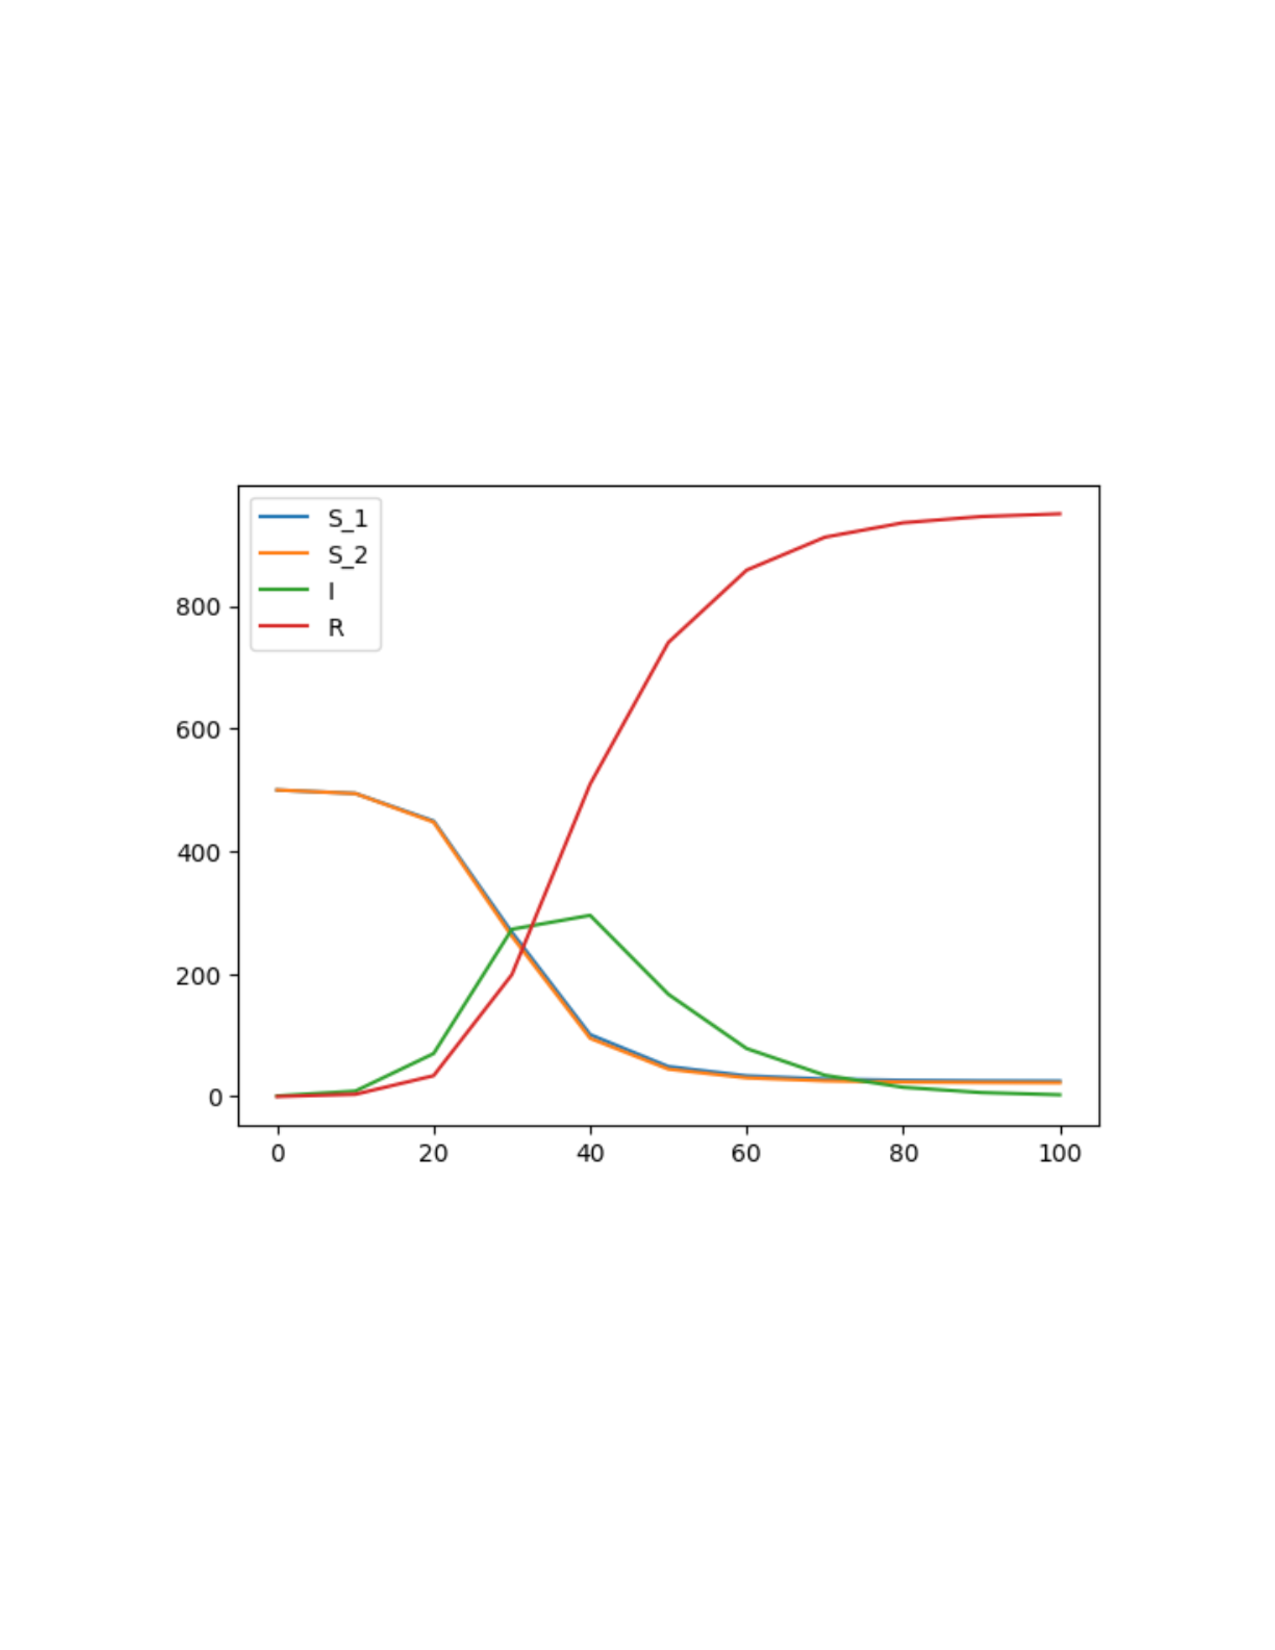
\includegraphics[width=\linewidth]{fig/sir/sir_stratified_sim.pdf}
%     \caption{\label{fig:sir_stratified_sim} Stratified SIR Model (top) and Simulation (bottom)}
% \end{figure}

% \section{Stratification Abstraction}
% The SIERHD model from the August monthly demo uses the model summarized by the Petrinet diagram in Figure \ref{fig:seirhd}.

\begin{figure}
    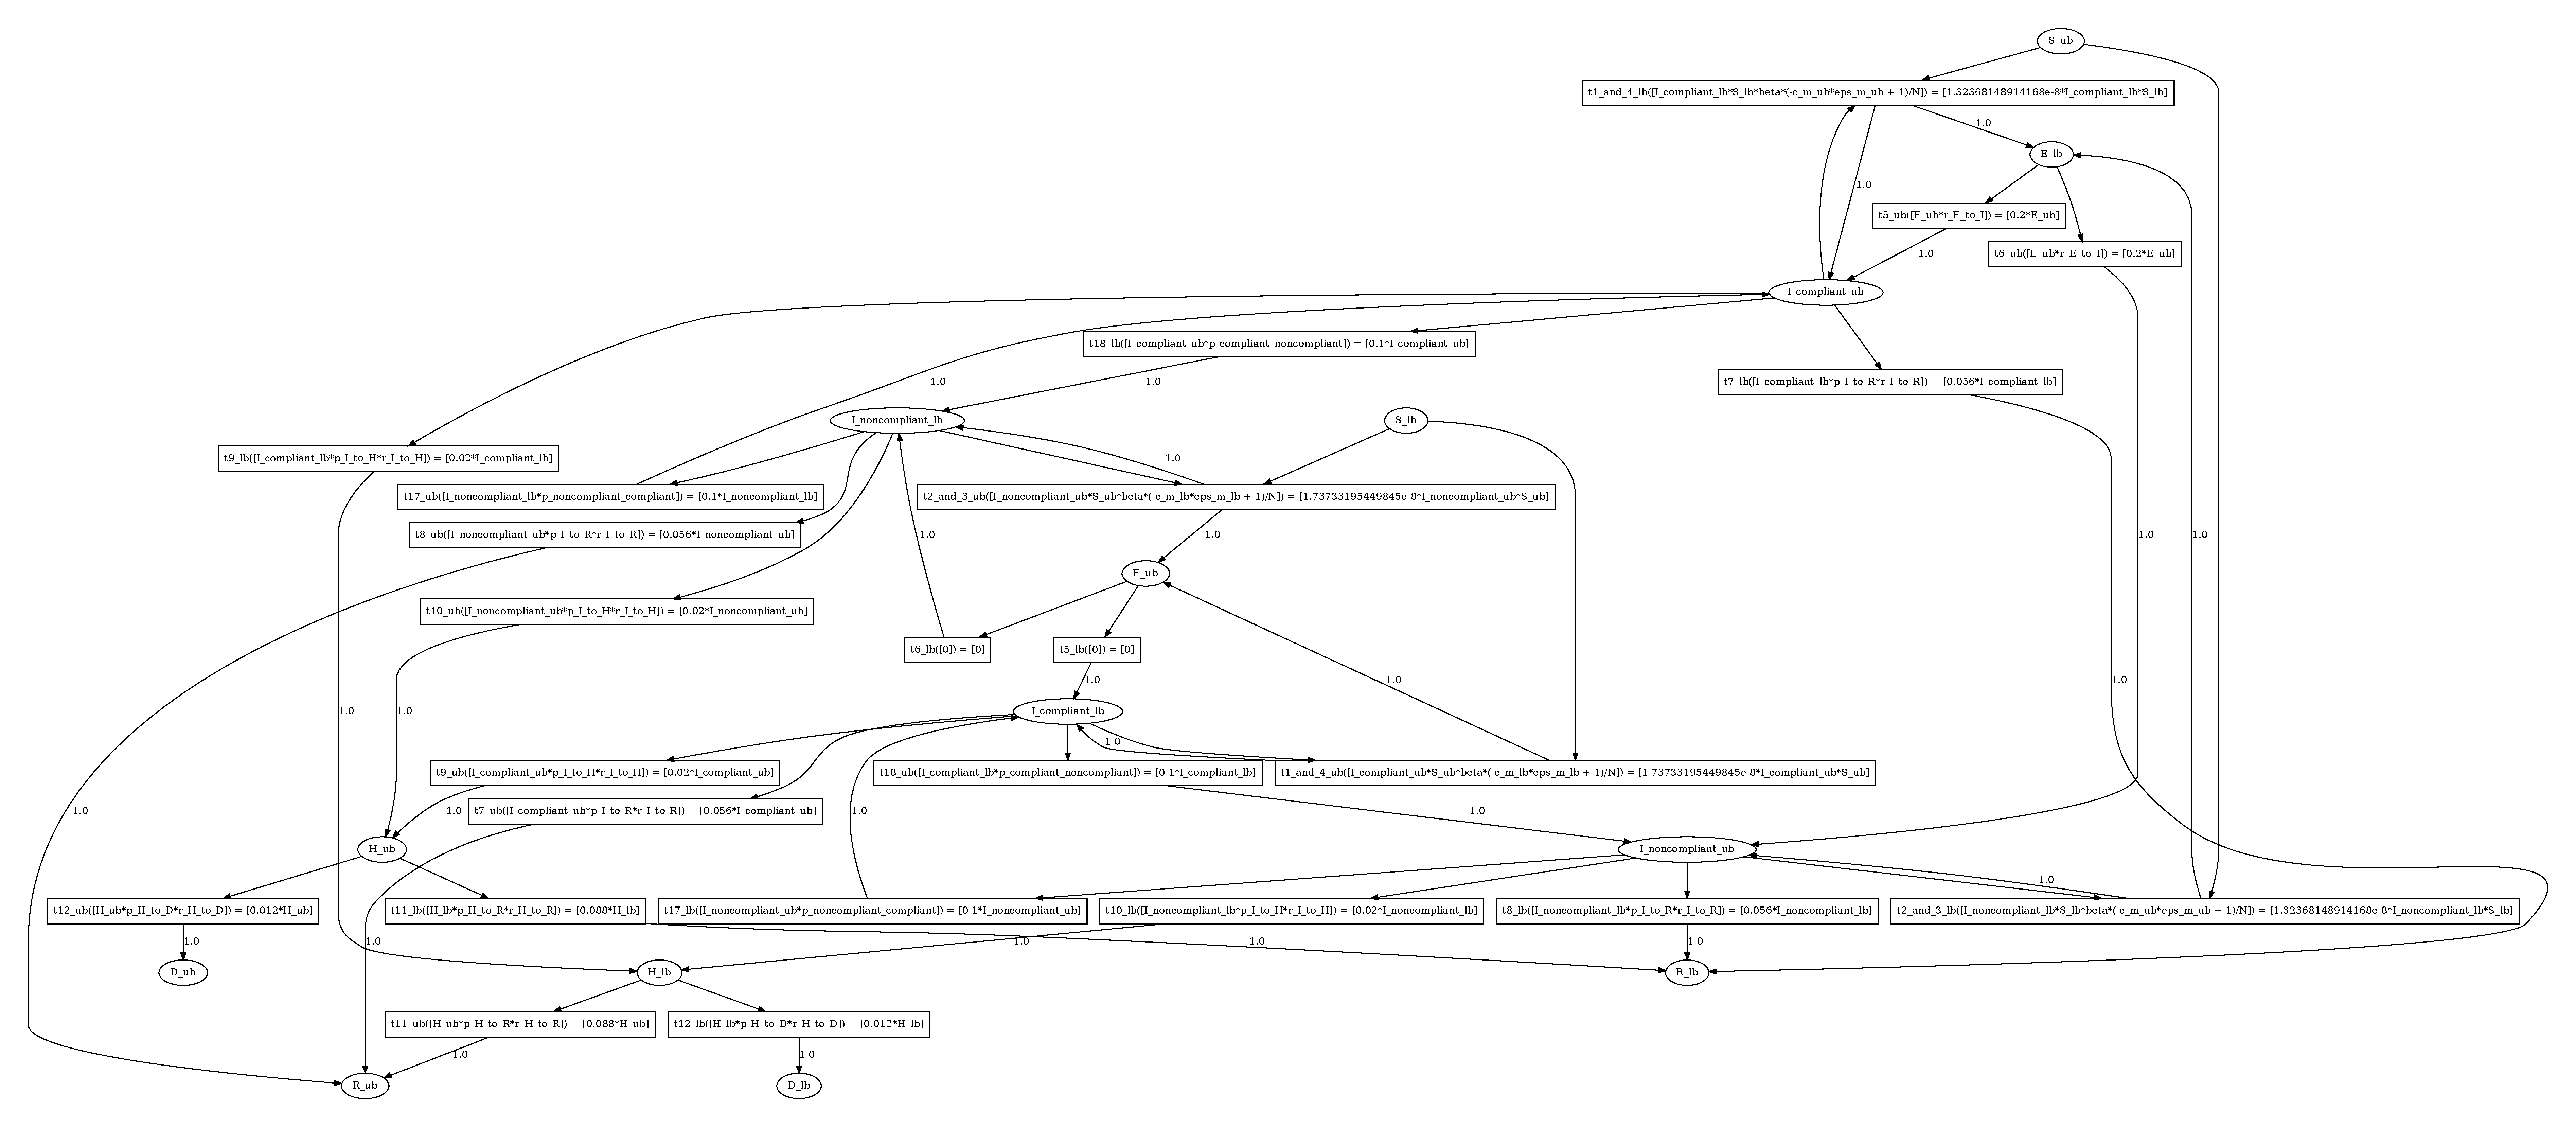
\includegraphics[width=\linewidth]{fig/seirhd-aug}
    \caption{\label{fig:seirhd} SEIRHD Model Petrinet}
\end{figure}

The following transitions connect the variables $S_c$, $S_{nc}$, $E_c$, $E_{nc}$, $I_c$, and $I_{nc}$, $R$, $H$, $D$:

\begin{eqnarray*}
    t_1: (I_c, S_c) &\xrightarrow[]{r_1}& (I_c, E_c) \\
    t_2: (I_{nc}, S_c) &\xrightarrow[]{r_2}& (I_{nc}, E_c)\\
    t_3: (I_{nc}, S_{nc}) &\xrightarrow[]{r_3}& (I_{nc}, E_{nc})\\
    t_4: (I_c, S_{nc}) &\xrightarrow[]{r_4}& (I_c, E_{nc})\\
    t_5: (E_c) &\xrightarrow[]{r_5}& (I_c)\\
    t_6:(E_{nc}) &\xrightarrow[]{r_6}& (I_{nc})\\
    t_7:(I_c) &\xrightarrow[]{r_7}& (R)\\
    t_8: (I_{nc}) &\xrightarrow[]{r_8}& (R)\\
    t_9:(I_c) &\xrightarrow[]{r_9}& (H)\\
    t_{10}:(I_{nc}) &\xrightarrow[]{r_{10}}& (H)\\
    t_{11}:(H) &\xrightarrow[]{r_{11}}& (R)\\
    t_{12}:(H) &\xrightarrow[]{r_{12}}& (D)\\
    t_{13}:(S_{nc}) &\xrightarrow[]{r_{13}}& (S_c)\\
    t_{14}:(S_c) &\xrightarrow[]{r_{14}}& (S_{nc})\\
    t_{15}:(E_{nc}) &\xrightarrow[]{r_{15}}& (E_c)\\
    t_{16}:(E_c) &\xrightarrow[]{r_{16}}& (E_{nc})\\
    t_{17}:(I_{nc}) &\xrightarrow[]{r_{17}}& (I_c)\\
    t_{18}:(I_c) &\xrightarrow[]{r_{18}}& (I_{nc})
\end{eqnarray*}

Abstracting this base model involves merging variables, such as $S_c$ and $S_{nc}$ into a composite variable $S$ where $S = S_c + S_{nc}$.  In this approach, a composite variable can represent any number of stratified copies of a variable (e.g., $S$ stratified by ten age groups). We also abstract the base model transitions so that their source and target variables are composite variables.  For example, if we define composite variables $S$, $I$, and $E$ for the corresponding stratified variables in the base model, then transitions $t_1$ to $t_4$ become the composite transition $t_{1:4}$:

\begin{eqnarray*}
    t_{1:4}:(I, S) &\xrightarrow[]{r_{1:4}}& (I, E)
\end{eqnarray*}

\noindent where $r_{1:4}$ is the composite rate of flow and $r_{1:4} = \sum_{i=1}^4 r_i$.  The composite rate of flow $r_{1:4}$ between the base variables due to the base transitions becomes difficult to track because we no longer separately model each base variable.  For example $r_1 = \frac{I_c S_c \beta(-c_{m_0}*\epsilon_{m_0} + 1)}{N}$, depends upon $I_c$ and $S_c$, and they are no longer variables in the abstract model.  We express $r_{1:4}$ in terms of the abstract variables by bounding it.  Bounding the rate expressions implies that we must also bound each of the variables.  We denote the upper and lower bounds with the $ub$ and $lb$ superscripts. 

For example, we express the rate $r_{1:4}$ with a pair of rates $r^{lb}_{1:4}$ and $r^{ub}_{1:4}$.  If we assume that the composite rate preserves the total flow between base model variables, we define bounds on the rate as follows: 

\begin{eqnarray*}
    S(t+dt) &=& S_c(t+dt) + S_{nc}(t+dt)\\
    &=& S_c(t) - (r_1+ r_2)dt  + S_{nc}(t) - (r_3+ r_4)dt\\
    &=& S(t) - (r_1+ r_2 +r_3+ r_4)dt\\
    &=& S(t) - \biggl(\frac{I_c S_c \beta(1-c_{m_0}\epsilon_{m_0})}{N}+\frac{I_{nc} S_c \beta(1-c_{m_1}\epsilon_{m_1} )}{N}+\\
    &&\qquad\qquad\frac{I_{nc} S_{nc} \beta(1-c_{m_2}\epsilon_{m_2} )}{N}+\frac{I_c S_{nc} \beta(1-c_{m_3}\epsilon_{m_3} )}{N}\biggl)dt\\
    &\leq& S(t) - \biggl(\frac{I_c S_c \beta(1-c^{ub}_{m}\epsilon^{ub}_{m}  )}{N}+\frac{I_{nc} S_c \beta(1-c^{ub}_{m}\epsilon^{ub}_{m})}{N}+\\
    &&\qquad\qquad\frac{I_{nc} S_{nc} \beta(1-c^{ub}_{m}\epsilon^{ub}_{m})}{N}+\frac{I_c S_{nc} \beta(1-c^{ub}_{m}\epsilon^{ub}_{m} )}{N}\biggl)dt\\
    &=& S(t) - \frac{\beta(1-c^{ub}_{m}\epsilon^{ub}_{m} )}{N}(I_c S_c +I_{nc} S_c +I_{nc} S_{nc} +I_c S_{nc} )dt\\
    &=& S(t) - \frac{\beta(1-c^{ub}_{m}\epsilon^{ub}_{m} )}{N}((I_c+I_{nc}) (S_c + S_{nc}) )dt\\
    &=& S(t) - \frac{\beta(1-c^{ub}_{m}\epsilon^{ub}_{m} )}{N}(IS)dt\\
    &\leq& S^{ub}(t) - \frac{I^{lb}S^{lb}\beta(1-c^{ub}_{m}\epsilon^{ub}_{m} )}{N}dt\\
    &=& S^{ub}(t+dt)
    % &&
\end{eqnarray*}

\noindent where the upper bound $S^{ub}(t+dt)$ assumes that the negative rate terms have minimal magnitude (i.e., the upper bound decreases by the least amount). The terms are minimal when they are replaced by the appropriate bounds $I^{lb}$, $S^{lb}$, $c^{ub}_{m}$, $\epsilon^{ub}_{m}$.  The lower bound $S^{ub}(t+dt)$ uses a similar approach, instead selecting bounds with a maximum magnitude and decreasing the lower bound by greatest amount.  Positive rate terms are handled similarly so that they are maximal when used to compute upper bounds and minimal for lower bounds.

The abstract model that de-stratifies the base model defines 12 compartments (lower and upper bound for each variable after defining the composite variables), and 12 transitions (lower and upper bound for each composite transition).  While the resulting model has fewer transitions, it has more compartments.  However, we would have constructed the same size abstraction for a stratified model with an arbitrary number of levels.  For example, if the base model used ten levels instead of two, then it would have 33 compartments and significantly more transitions.  

We developed two abstract models from the base model.  The first, as described above, de-stratifies the $S$, $E$, and $I$ variables.  The second, de-stratifies only $S$ and $E$, allowing $I$ to remain stratified.  

\begin{figure}
    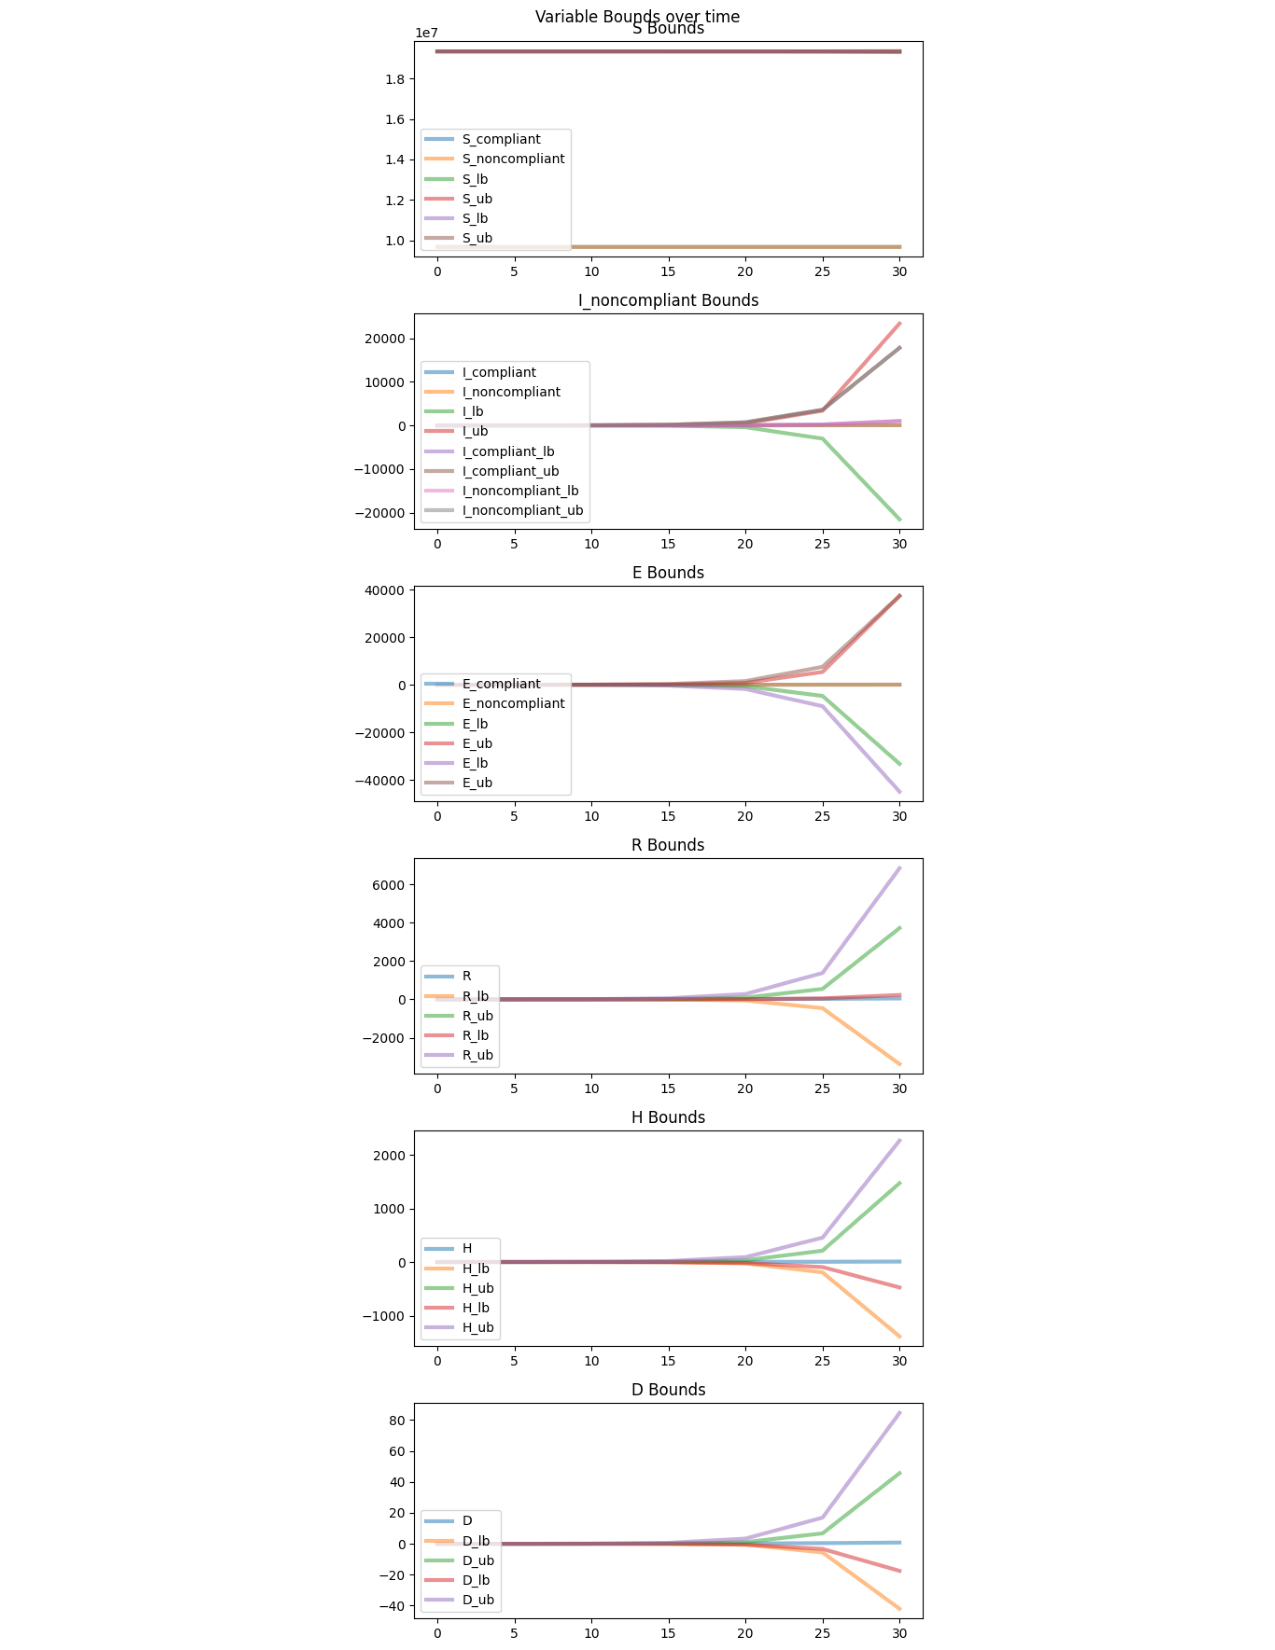
\includegraphics[width=\linewidth]{fig/seirhd_bounds.pdf}
    \caption{\label{fig:seirhd-bounds} SEIRHD Model Bounds}
\end{figure}

Figure \ref{fig:seirhd-bounds} illustrates the bounds computed by simulating the base and abstract models with FUNMAN.  Each subplot is one compartment variable, and each series is one of the bounds or base model value.  For example, the second plot illustrates $I$, which includes:
\begin{itemize}
    \item Base model: $I$\_compliant and $I$\_\text{noncompliant}, 
    \item De-stratified $S$, $E$, and $I$:  $I$\_\text{lb} and $I$\_\text{ub},
     \item De-stratified $S$, and $E$:  $I$\_compliant\_lb, $I$\_compliant\_ub,$I$\_noncompliant\_lb and $I$\_noncompliant\_ub,
\end{itemize}
The abstractions provide different bounds for each variable.  In general, as abstraction increases, the model will provide looser bounds, but with a smaller model.  Using abstraction refinement techniques, it is possible to start with an abstract model and only refine the relevant variables.  Selectively refining models will trade off multiple abstract model simulations against a single, potentially large model simulation.  In cases where the bounds are enough to answer a query (or check a constraint), the abstract model simulation can lead to significant scale up.  

% \section{Parameter Synthesis as Abstraction Refinement}

% Parameter synthesis involves labeling regions of a parameter space as safe or unsafe.  This can be formulated as an expression:

% \begin{align}
%     \label{eqn:formulation1}\tag{F1}
%      & \exists \posregion \subseteq \reals^n \forall \point \in \posregion. \model(\point) \wedge \query(\point)         & // & \text{true}  \\
%     \label{eqn:formulation2}\tag{F2}
%      & \exists \negregion \subseteq \reals^n \forall \point \in \negregion. \neg \model(\point) \vee \neg \query(\point) & // & \text{false}
%     % \label{eqn:formulation3}
%     %  & \exists \irrelevantregion \subseteq \reals^n \forall \point \in \irrelevantregion. \neg \model(\point)         & // & \text{irrelevant}
% \end{align}
% \noindent where each point $\point$ is an $n$-dimensional vector.  We refer to $\posregion$ and $\negregion$ as the respective ``true'' and ``false'' sets.  We call the pair $(\posregion, \negregion)$ the parameter space of $\model$ and $\query$.



% In addition to the parameters comprising the parameter space, the model includes a set of state variables $V$.  The model defines (via ODE or PDE equations) the state $S$ at various points in time and space.  We augment the state to include the (constant or piece-wise constant) model parameters, as well as structural parameters describing the time horizon and step size.

% An abstraction of the state space groups states into abstract states, and defines abstract transitions between abstract states.  An abstract transition between abstract states indicates that there exists at least one transition between states of the respective abstract states.  

\end{document}